%====================================================
%
% Author: Dipl.-Inf. Xavier NOUMBISSI NOUNDOU, Ph.D.-Candidate
% Email:  xnoundou7@gmail.com
%
%====================================================
\documentclass[10pt, a4paper]{bookest}
\NeedsTeXFormat{LaTeX2e}
\makeindex

%---------------------------- PACKAGE INCLUSION -------------------------------
% This group renders characters clearer and more precise

\RequirePackage[bitstream-charter,cal,expert]{mathdesign}
\RequirePackage{makeidx}
\RequirePackage{latexsym}

\usepackage{geometry} % to change the page dimensions
\geometry{a4paper,
		  %showframe=true,
		  %margin=3cm,
		  %a4paper,
		  %total={170mm,257mm},
		  top=4.15em,
		  left=5.5em,
		  right=5.5em,
		  bottom=3.39em
		  }

\usepackage[default]{cantarell}
\usepackage{graphicx}
\usepackage[french]{babel}
\usepackage{xspace}
\usepackage[parfill]{parskip} % Activate to begin paragraphs with an empty line rather than an indent
\usepackage{paralist} % very flexible & customisable lists (eg. enumerate/itemize, etc.)
\usepackage{listings} % for lstset definitions
\usepackage{url}
\usepackage{subfig} % make it possible to include more than one captioned figure/table in a single float
\usepackage{epsfig}
\usepackage{booktabs}
%\usepackage{enumitem} %funny itemize icons
\usepackage{verbatim}

\usepackage{amsmath}
\newcommand{\mathbold}[1]{\text{\textbf{#1}}}

\usepackage{xcolor}
\definecolor{forestgreen}{RGB}{2,160,70}    
\definecolor{mediumblue}{RGB}{7,43,205}    
\definecolor{firebrickred}{RGB}{178,34,34}
\definecolor{listingray}{gray}{0.9}
\definecolor{lbcolor}{rgb}{0.9,0.9,0.9}
\definecolor{darkgreen}{rgb}{0,0.35,0}
\definecolor{medgreen}{rgb}{0,0.5,0}
\definecolor{lightgreen}{rgb}{0.5,0.7,0.5}
\definecolor{pmcolour}{rgb}{0.5,0.7,0.5}
\definecolor{medgrey}{rgb}{0.6,0.6,0.6}
\definecolor{purplish}{rgb}{0.4,0,0.6}
\definecolor{brightred}{rgb}{1,0.2,0.2}

\newcommand{\diplominformatiker}{Diplom--Informatiker\xspace}

\newcommand{\diplinfn}{Dipl.--Inf.\xspace}

\newcommand{\pos}{syst\`eme--logiciel ERP\xspace}

\newcommand{\yerenlabs}{\textsc{Yeroth--R\&D}\xspace}

\newcommand{\yerenpos}{\textcolor{yerenColorBlue}{\sc YEROTH--ERP--$3.0$}\xspace}

\newcommand{\myfullacademicname}{Xavier NOUMBISSI NOUNDOU, Ph.D. (ABD)\xspace}

\usepackage{hyperref}
\hypersetup{
    colorlinks,
	pagebackref,
    citecolor=medgreen,
    linkcolor=purplish,
    breaklinks,
    pdftex,
    bookmarks,
    plainpages=false,
	pdftitle={Manuel de l'Utilisateur ''Administrateur'' de YEROTH-ERP (version $3.0$)
				par \myfullacademicname},
    pdfauthor={Xavier NOUMBISSI NOUNDOU, Ph.D. (ABD)}
}

%--------------------------------------------------------------------------------

%---------------------------- COMMANDS DEFINITION -------------------------------
\newcommand{\tool}[1]{\texttt{\textbf{#1}}\xspace}
\newcommand{\UUT}{Unit Under Test\xspace}
\newcommand{\annotation}[1]{ \texttt{\textbf{#1}}\xspace}
\newcommand{\junit}{\texttt{\textbf{JUnit}}\xspace}
\newcommand{\company}[1]{\textbf{#1}\xspace}
\newcommand{\diplinf}{\textsc{Dipl.-Inf.}\xspace}
\newcommand{\saint}{\textbf{\textsc{SAINT}}\xspace}

\newcommand{\emphbf}[1]{\textbf{#1}\xspace}
\newcommand{\emphit}[1]{\emph{\textit{#1}}\xspace}
\newcommand{\mycheckmark}[1]{\textcolor{#1}{$\checkmark$}\xspace}
\newcommand{\mytimes}[1]{\textcolor{#1}{$\times$}\xspace}
\newcommand{\boldsc}[1]{\textbf{\textsc{#1}}\xspace}

\newcommand{\myenumitem}[1]{\emph{#1}\xspace}

\newcommand{\bergmann}{Bergmann Automaten GmbH\xspace}
\newcommand{\siemens}{\textsc{Siemens} Medical Solutions\xspace}
\newcommand{\watformlab}{Watform Lab\xspace}
\newcommand{\uwaterloo}{University of Waterloo\xspace}


\newcommand{\javalanguage}{\emph{Java}\xspace}
\newcommand{\vmodel}{\emph{V-Model}\xspace}

\newcommand{\yeren}{\textsc{yeroth--erp--3.0}\xspace}
\newcommand{\yerenalert}{\emph{yeroth--erp--alert--3.0}\xspace}
\newcommand{\mysql}{MySQL\xspace}
\newcommand{\depot}{d\'ep\^ot\xspace}
\newcommand{\depots}{d\'ep\^ots\xspace}
\newcommand{\bouton}[1]{"\textbf{#1}"\xspace}
\newcommand{\field}[1]{"\emph{\textbf{#1}}"\xspace}

\newcommand{\role}{r\^ole\xspace}
\newcommand{\roles}{r\^oles\xspace}
\newcommand{\manager}{\emph{Manager}\xspace}
\newcommand{\gestionairedestocks}{\emph{GestionaireDeStocks}\xspace}
\newcommand{\magasinier}{\emph{Magasinier}\xspace}
\newcommand{\caissier}{\emph{Caissier}\xspace}
\newcommand{\admin}{\emph{Administrateur}\xspace}

\newcommand{\qt}{Qt$5.7$\xspace}

\newcommand{\managerb}{\emph{\textbf{Manager}}\xspace}
\newcommand{\gestionairedestocksb}{\emph{\textbf{GestionaireDeStocks}}\xspace}
\newcommand{\caissierb}{\emph{\textbf{Caissier}}\xspace}
\newcommand{\administrateurb}{\emph{\textbf{Administrateur}}\xspace}
\newcommand{\magasinierb}{\emph{\textbf{Magasinier}}\xspace}

\newcommand{\utilisateurs}
	{\textcolor{blue}{\textbf{\emph{R\^oles ayant acc\`es \`a la fonctionalit\'e}}}\xspace}
	
\newcommand{\optionel}{\textcolor{firebrickred}{\textbf{\emph{[optionel]}}}\xspace}

\newcommand{\lienmagasinier}{\magasinier~\ref{sec:utilisateurs-lemagasinier}\xspace}
\newcommand{\liencaissier}{\caissier~\ref{sec:utilisateurs-lecaissier}\xspace}
\newcommand{\lienadmin}{\admin~\ref{sec:utilisateurs-ladministrateur}\xspace}
\newcommand{\lienmanager}{\manager~\ref{sec:utilisateurs-lepatron}\xspace}
\newcommand{\yerenfield}[1]{\textbf{\emph{#1}}\xspace}
\newcommand{\procparagraph}[1]
	{\paragraph{ \mycheckmark{forestgreen} \emph{\textcolor{forestgreen}{#1}}}}

\newcommand{\xavier}{Xavier NOUMBISSI NOUNDOU\xspace}

\newcommand{\reference}{r\'ef\'erence\xspace}

\newcommand{\cmup}{\textbf{CMUP}\xspace}
\newcommand{\dpfdpo}{\textbf{DEF\_DEO}\xspace}
\newcommand{\fifo}{\textbf{FIFO}\xspace}
\newcommand{\lifo}{\textbf{LIFO}\xspace}

\newcommand{\fenetre}{fen\^etre\xspace}
\newcommand{\uielemone}[1]{\textcolor{medgreen}{\emph{#1}}\xspace}
\newcommand{\uielemtwo}[1]{\textcolor{mediumblue}{\texttt{#1}}\xspace}

\newcommand{\nxsection}[1]{\section{#1}\xspace}
\newcommand{\nxsubsection}[1]{\subsection{#1}\xspace}
\newcommand{\chapintro}[1]{\textcolor{purplish}{\emph{#1}}\xspace}

%\usepackage{makeidx} % Used to generate the index
%\makeindex % Generate the index which is printed at the end of the document

%--------------------------------------------------------------------------------

\usepackage[T1]{fontenc}
\newcommand{\changefont}[3]{
\fontfamily{#1} \fontseries{#2} \fontshape{#3} \selectfont}
\changefont{cmss}{m}{n}

% Set font to avant-garde
%\renewcommand*\rmdefault{pag}

%Remove widows and orphants
\clubpenalty = 10000
\widowpenalty = 10000
\displaywidowpenalty = 10000

\begin{document}
\frontmatter\pagestyle{plain}
\title{\textcolor{medgreen}{\textsc{Syst\`eme--Logiciel ERP
		\\ \vspace*{1.5cm}(\yeren)\\}
		\vspace*{3cm}
	Manuel de l'Utilisateur\\ \vspace{1em} << Administrateur >>}}

\begin{titlepage}
\maketitle
\vspace{\stretch{2}}
\centering
\copyright\ \textsc{\myfullacademicname}
\end{titlepage}

% TABLE OF CONTENTS
\cleardoublepage
\phantomsection
\addcontentsline{toc}{chapter}{\contentsname}
\begingroup
\color{medgreen}
\tableofcontents
\endgroup

% LIST OF TABLES
\cleardoublepage
\phantomsection
\addcontentsline{toc}{chapter}{\listtablename}
\begingroup
\color{medgreen}
\listoftables
\endgroup

% LIST OF FIGURES
\cleardoublepage
\phantomsection
\addcontentsline{toc}{chapter}{\listfigurename}
\begingroup
\color{medgreen}
\listoffigures
\endgroup

\cleardoublepage
\phantomsection
\addcontentsline{toc}{chapter}{\`A propos de l'auteur}
\chapter*{\`A propos de l'auteur}\label{chap:biography}
\index{\`a propos de l'auteur}
\index{biographie de l'auteur}

\begin{figure}[!htpb]
\centering
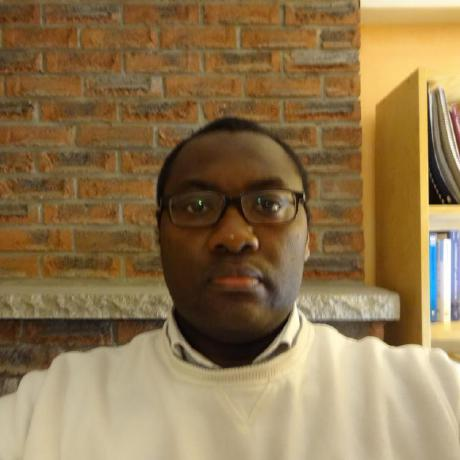
\includegraphics[scale=0.63]{images/XavierNOUNDOU-2}
\caption{Portrait de Xavier}~\label{fig:xaviernoumbis}
\end{figure}


\mainmatter

\chapter{Introduction}\label{chap:introduction}

\yeren est un syst\`eme logiciel de gestion des
stocks et de gestion des ventes. Il permet
d'ex\'ecuter des mouvements de stocks, et de
vendre des articles en stocks.

Une entreprise doit poss\'eder au minimum d'un stock
d'articles, d'un d\'ep\^ot ou d'une boutique pour utiliser
\yeren de fa\c{c}on efficace.\\

\begin{figure}[!htpb]
	\centering
	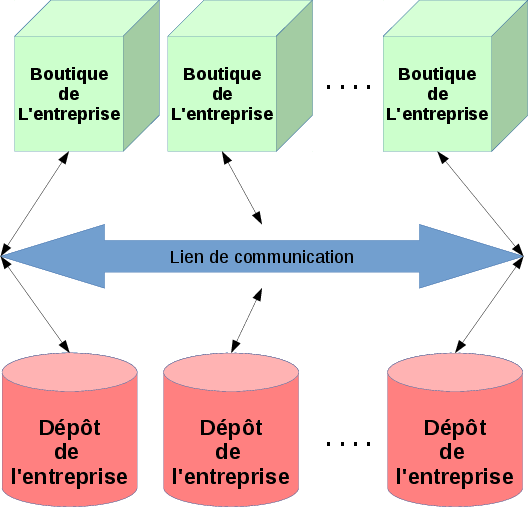
\includegraphics[scale=0.63]{images/architecture-enterprise-yeren.png}
	\caption{Un mod\`ele d'architecture d'une entreprise}\label{fig:architecture-enterprise-yeren}
\end{figure}

La figure~\ref{fig:architecture-enterprise-yeren} illustre
un mod\`ele g\'en\'erique d'entreprise o\`u les d\'ep\^ots
et les boutiques de l'entreprise sont en communication.

Les activit\'es principales de l'entreprise sont les suivantes:
\begin{enumerate}[1)]
	\item \emphbf{les sorties de stocks:} sortie d'articles
		d'une unit\'e (boutique ou d\'ep\^ot) pour r\'eception par un client
	\item \emphbf{les transferts de stocks:} mouvement d'articles
		d'une unit\'e vers une autre unit\'e
	\item \emphbf{les ventes d'articles:} un client ach\`ete
		des articles qui lui sont ensuite remis.\\
\end{enumerate}

\yeren permet d'accomplir les t\^aches de gestion
des stocks et de gestion des ventes suivantes:
\begin{enumerate}[1)]
	\item \myenumitem{cr\'eer des alertes sur des p\'eriodes de temps}	
	\item \myenumitem{cr\'eer des alertes sur des quantit\'e en stocks}	
	\item \myenumitem{entrer un stock}
	\item \myenumitem{lister les stocks}
	\item \myenumitem{modifier un stock}
	\item \myenumitem{supprimer un stock}	
	\item \myenumitem{rechercher des articles ou des stocks}
	\item \myenumitem{transf\'erer des articles ou des stocks}	
	\item \myenumitem{vendre des articles}	
	\item \myenumitem{visualiser les \'etats de transactions d'articles
		(sorties ou transferts de stocks)}
	\item \myenumitem{acc\'eder aux tableaux de bords}
	\item \myenumitem{visualiser les \'etats de ventes d'articles}.\\
\end{enumerate}

\newpage

\section{Acc\`es au manuel de l'utilisateur}

La figure~\ref{fig:fenetre-principale-utilisateur-non-enregistre}
illustre la fen\^etre d'accueil de \yeren sans aucun utilisateur
enregistr\'e.\\

\begin{figure}[!htbp]
\centering
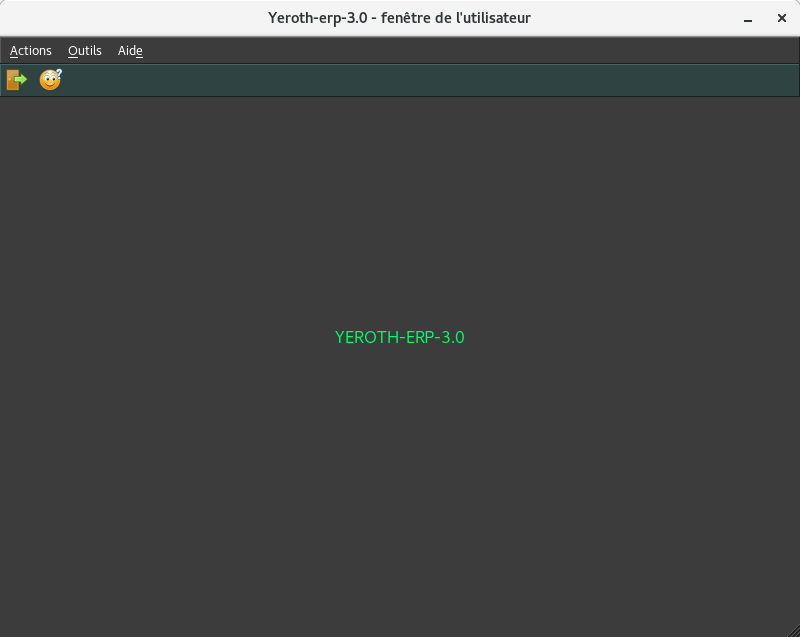
\includegraphics[scale=0.63]{images/yeren-fenetre-principale.png}
\caption{La fen\^etre d'acceuil sans aucun utilisateur enregistr\'e.}
\label{fig:fenetre-principale-utilisateur-non-enregistre}
\end{figure}

Il est requis qu'un utilisateur soit enregistr\'e
dans \yeren afin d'avoir acc\`es au manuel de l'utilisateur.

L'utilisateur de \yeren doit accomplir les op\'erations
suivantes afin d'avoir acc\`es au manuel de l'utilisateur:
\begin{enumerate}[1)]
	\item \`a partir de la fen\^etre d'accueil
		(voir figure~\ref{fig:fenetre-principale-utilisateur-non-enregistre}),
		cliquez sur le menu d\'eroulant '\textbf{Aide}'
	\item ensuite cliquez sur le lien '\textbf{Manuel de l'utilisateur (PDF)}'.
\end{enumerate}

\section{Structure de ce manuel de l'utilisateur}
Ce manuel de  l'utilisateur de \yeren est structur\'e
comme suit:

\begin{itemize}[\mycheckmark{purplish}]
	\item le chapitre~\ref{chap:utilisateurs} d\'ecrit
	les utilisateurs de \yeren et leurs \roles. 
	     
	\item le chapitre~\ref{chap:gestion-stocks} explicite
	les fonctionalit\'es de gestion des stocks

	\item le chapitre~\ref{chap:gestion-des-achats} parle
	de la gestion des achats
	
	\item le chapitre~\ref{chap:systeme-dalertes}
	pr\'esente le syst\`eme d'alertes sur les stocks
	
	\item le chapitre~\ref{chap:vendre} d\'ecrit comment
	conclure des ventes d'articles
	
	\item le chapitre~\ref{chap:sortir-articles} d\'ecrit
	comment proc\'eder \`a des sorties et transferts de stocks
	
	\item le chapitre~\ref{chap:vente} explicite comment
	rechercher et imprimer les \'etats de ventes d'articles
	
	\item le chapitre~\ref{chap:etats-des-sorties} explicite
	comment rechercher et imprimer les \'etats de sorties ou
	transferts d'articles
	
	\item le chapitre~\ref{chap:tableaux-de-bord} discute
	de la recherche et de la g\'en\'eration des rapports
	commerciaux de l'entreprise
	
	\item le chapitre~\ref{chap:informations-generales}
	explique comment avoir acc\`es aux d\'etails de
	l'utilisateur enregistr\'e, aux informations commerciales
	de l'entreprise, et enfin \`a la version de \yeren que
	l'on utilise
	
	\item le chapitre~\ref{chap:administration-logiciel}
	traite de l'administration du logiciel

	\item le chapitre~\ref{chap:problemes-connues}
	discute des probl\`emes connues de \yeren
	
	\item enfin, le chapitre~\ref{chap:conclusion} conclut
	ce manuel d'utilisation.
\end{itemize}


\chapter{Les R\^oles et Les Utilisateurs}\label{chap:utilisateurs}
\index{types de \roles}

\utilisateurs: \lienadmin, \liencaissier, \lienmagasinier, \lienpatron.\\

\chapintro{Ce chapitre d\'ecrit les diff\'erents types d'utilisateurs de
\yeren: \admin, \magasinier, \caissier, et \patron.}

\nxsection{Introduction}\label{sec:utilisateurs-introduction}

\yeren maintient les donn\'ees suivantes pour chaque utilisateur:
\begin{enumerate}[1)]
	\item l'\'email \optionel
	\item la bo\^ite postale
	\item le date de naissance \optionel
	\item le lieu de naissance \optionel
	\item la localisation (le site de l'entreprise o\`u l'employ\'e
	      est en fonction). Cette valeur ne peut \^etre \'edit\'ee.
	      Sa valeur est automatiquement remplie \`a partir de la
	      license d'installation.
	\item le nom
	\item le num\'ero de t\'el\'ephone 1 \optionel
	\item le num\'ero de t\'el\'ephone 2 \optionel
	\item le pays \optionel
	\item le pr\'enom	
	\item la province / \'etat
	\item le r\^ole dans \yeren (\admin, \magasinier, \caissier, ou \patron)
	\item le titre (Dr., Me., Mlle, Mme, Mr, Pr., Prof.)
	\item la ville \optionel
\end{enumerate}

\newpage

\nxsection{Le r\^ole ''Administrateur''}\label{sec:utilisateurs-ladministrateur}
\index{administrateur}
\index{LAdministrateur}

La figure~\ref{fig:fenetre-principale-admin} illustre la
fen\^etre d'acceuil d'un utilisateur avec le \role \admin,
apr\`es qu'il se soit enregistr\'e dans \yeren.\\

\begin{figure}[!htbp]
\centering
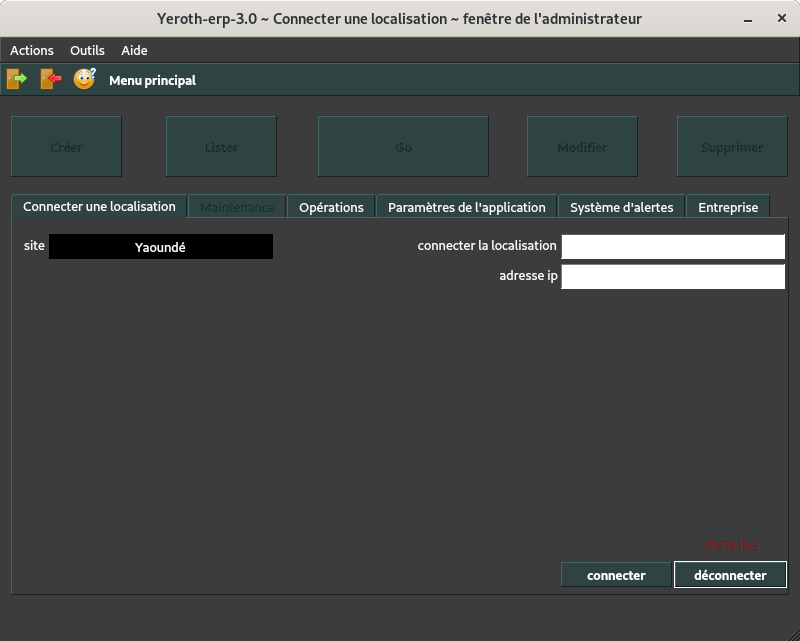
\includegraphics[scale=0.63]{images/yeroth-fenetre-administrateur.png}
\caption{La fen\^etre d'acceuil d'un administrateur.}
\label{fig:fenetre-principale-admin}
\end{figure}

Un utilisateur avec le \role "\admin" assume les
t\^aches de cr\'eer et de maintenir les objets suivants:
\begin{enumerate}[1)]
	\item les alertes (sur une p\'eriode de temps, ou sur une quantit\'e en stock)
	%\item les bons de commande
	\item les cat\'egories d'articles
	\item les clients
	\item les comptes utilisateurs
	\item les fournisseurs				
	\item les localisations (une localisation est un site de
	      l'entreprise o\`u se trouve un ou plusieurs stocks).\\   
\end{enumerate}

\newpage

\nxsection{Le r\^ole ''Manager''}\label{sec:utilisateurs-lepatron}
\index{patron}
\index{LePatron}

La figure~\ref{fig:yeren-fenetre-patron} illustre la fen\^etre
d'acceuil d'un utilisateur avec le \role \patron, 
apr\`es qu'il se soit enregistr\'e dans \yeren.\\

\begin{figure}[!htbp]
\centering
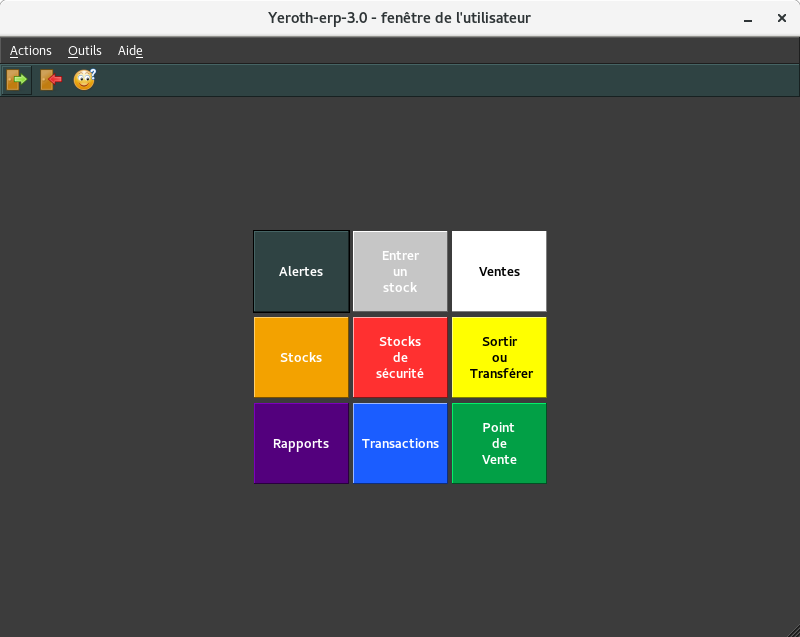
\includegraphics[scale=0.63]{images/yeren-fenetre-patron.png}
\caption{La fen\^etre d'acceuil d'un ''manager''}
\label{fig:yeren-fenetre-patron}
\end{figure}

Un utilisateur de \yeren avec le \role "\patron" a
acc\`es \`a toutes les fonctionalit\'es de \yeren. Il
cumule les t\^aches de d'administrateur, de magasinier,
et de caissier.

Le \role \patron est le seul \`a donner acc\`es aux
informations des ventes dans leurs totalit\'es, ainsi
qu'\`a la g\'en\'eration et \`a la consultation des
rapports commerciaux.

Le \role \patron est le seul \`a pouvoir consulter toutes
les alertes re\c{c}ues par les autres utilisateurs, et
\`a pouvoir les supprimer.

\newpage

\nxsection{Le r\^ole ''GestionaireDeStocks''}\label{sec:utilisateurs-gestionairedestocks}
\index{gestionaire de stocks}
\index{GestionaireDeStocks}

La figure~\ref{fig:yeren-fenetre-gestionairedestocks} illustre
la fen\^etre d'acceuil d'un utilisateur avec le \role \gestionairedestocks, 
apr\`es qu'il se soit enregistr\'e dans \yeren.\\

\begin{figure}[!htbp]
\centering
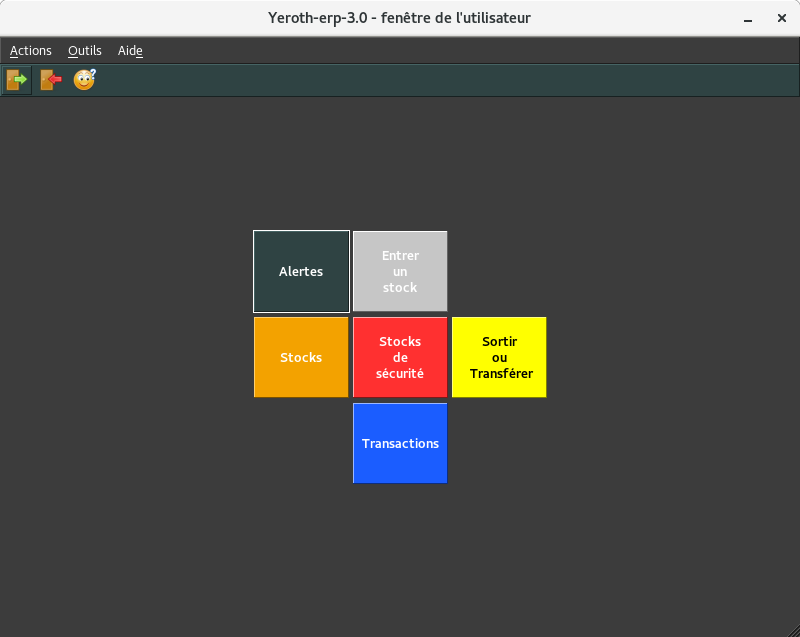
\includegraphics[scale=0.63]{images/yeren-fenetre-gestionairedestocks.png}
\caption{La fen\^etre d'acceuil d'un gestionaire de stocks}
\label{fig:yeren-fenetre-gestionairedestocks}
\end{figure}

\newpage

\nxsection{Le r\^ole ''Magasinier''}\label{sec:utilisateurs-lemagasinier}
\index{magasinier}
\index{LeMagasinier}

La figure~\ref{fig:yeren-fenetre-magasinier} illustre
la fen\^etre d'acceuil d'un utilisateur avec le
\role \magasinier, apr\`es qu'il se soit enregistr\'e
dans \yeren.\\

\begin{figure}[!htbp]
\centering
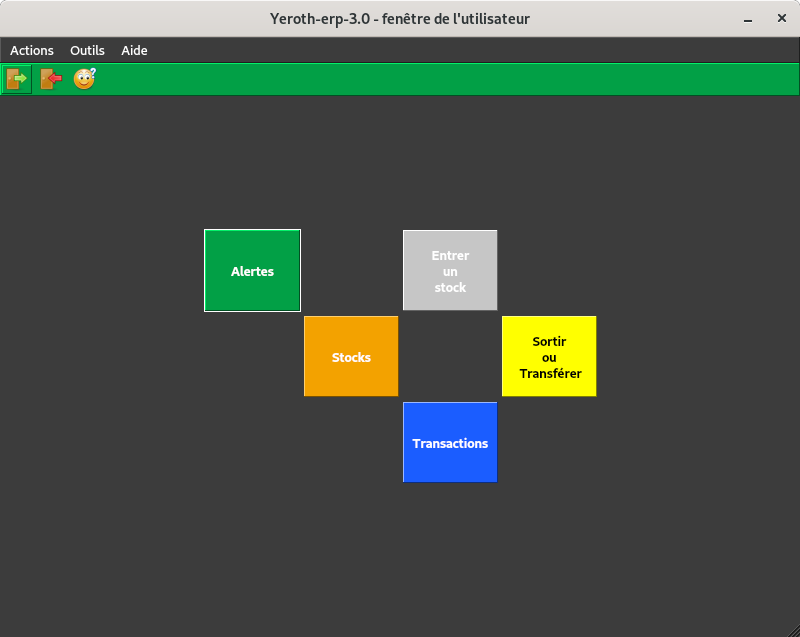
\includegraphics[scale=0.63]{images/yeren-fenetre-magasinier.png}
\caption{La fen\^etre d'acceuil d'un magasinier.}
\label{fig:yeren-fenetre-magasinier}
\end{figure}

Un utilisateur de \yeren avec le \role "\magasinier" assume les
t\^aches suivantes:
\begin{enumerate}[1)]
	\item lister des stocks
	\item modifier un stock
	\item rechercher des articles / stocks
	\item rechercher des transactions 
		(sorties de stocks ou transferts de stocks)
	\item sortir des articles / stocks
	\item supprimer un stock
	\item transf\'erer un stock
	\item visualiser des transactions
	(sorties de stocks ou transferts de stocks).\\
\end{enumerate}

\magasinier n'a pas acc\`es aux fonctions
\bouton{Administration}, \bouton{Ventes},
\bouton{Rapports}, et \bouton{Vendre}.

On remarque sur la Figure~\ref{fig:yeren-fenetre-magasinier}
que les boutons \bouton{Administration}, \bouton{Ventes},
\bouton{Rapports}, et \bouton{Vendre} sont d\'esactiv\'es.
	
\newpage

\nxsection{Le r\^ole ''Caissier''}\label{sec:utilisateurs-lecaissier}
\index{caissier}
\index{LeCaissier}

La figure~\ref{fig:fenetre-principale-caissier} illustre la
fen\^etre d'acceuil d'un utilisateur avec le \role \caissier,
apr\`es qu'il se soit enregistr\'e dans \yeren.\\

\begin{figure}[!htbp]
\centering
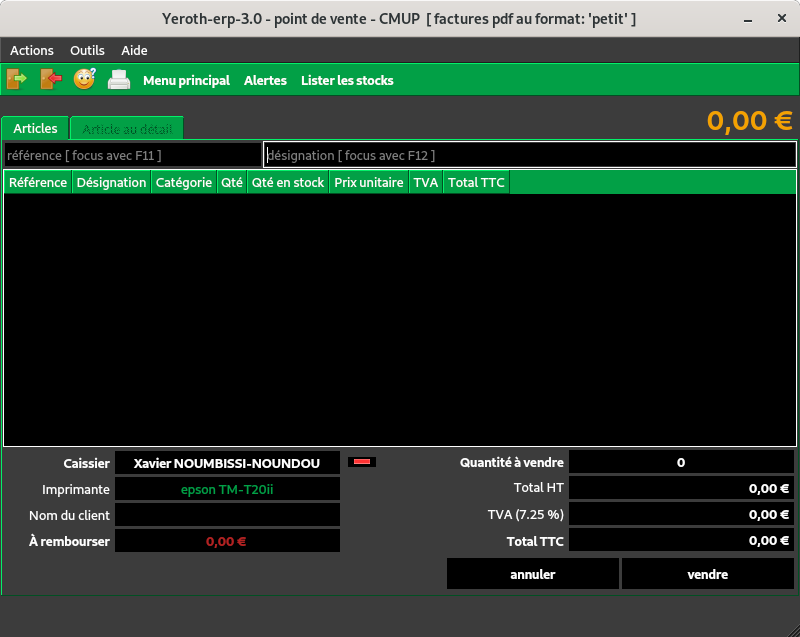
\includegraphics[scale=0.63]{images/yeren-fenetre-caissier.png}
\caption{La fen\^etre d'acceuil d'un caissier.}
\label{fig:fenetre-principale-caissier}
\end{figure}

Un utilisateur de \yeren avec le \role "\caissier" assume
les t\^aches suivantes:
\begin{enumerate}[1)]
	\item lister les stocks \`a partir de l'interface de vente	
	\item visualiser une facture proforma		
	\item imprimer une facture proforma
	\item vendre un ou plusieurs stocks (ou articles).\\
\end{enumerate}

\chapter{Les Informations G\'en\'erales}\label{chap:informations-generales}

\utilisateurs: \lienadmin, \liencaissier, \lienmagasinier, \lienmanager.\\

\chapintro{Ce chapitre d\'ecrit comment avoir acc\`es aux
informations publiques de l'entreprise et de \yeroth
(ex.: le si\`ege social de l'entreprise, la version
de \yeroth utilis\'ee, etc).}

\nxsection{Voir les d\'etails de l'utilisateur avec lequel
			on s'est enregistr\'e}
\index{voir les d\'etails de l'utilisateur avec lequel
		on s'est enregistr\'e}

\begin{figure}[!htbp]
	\centering
	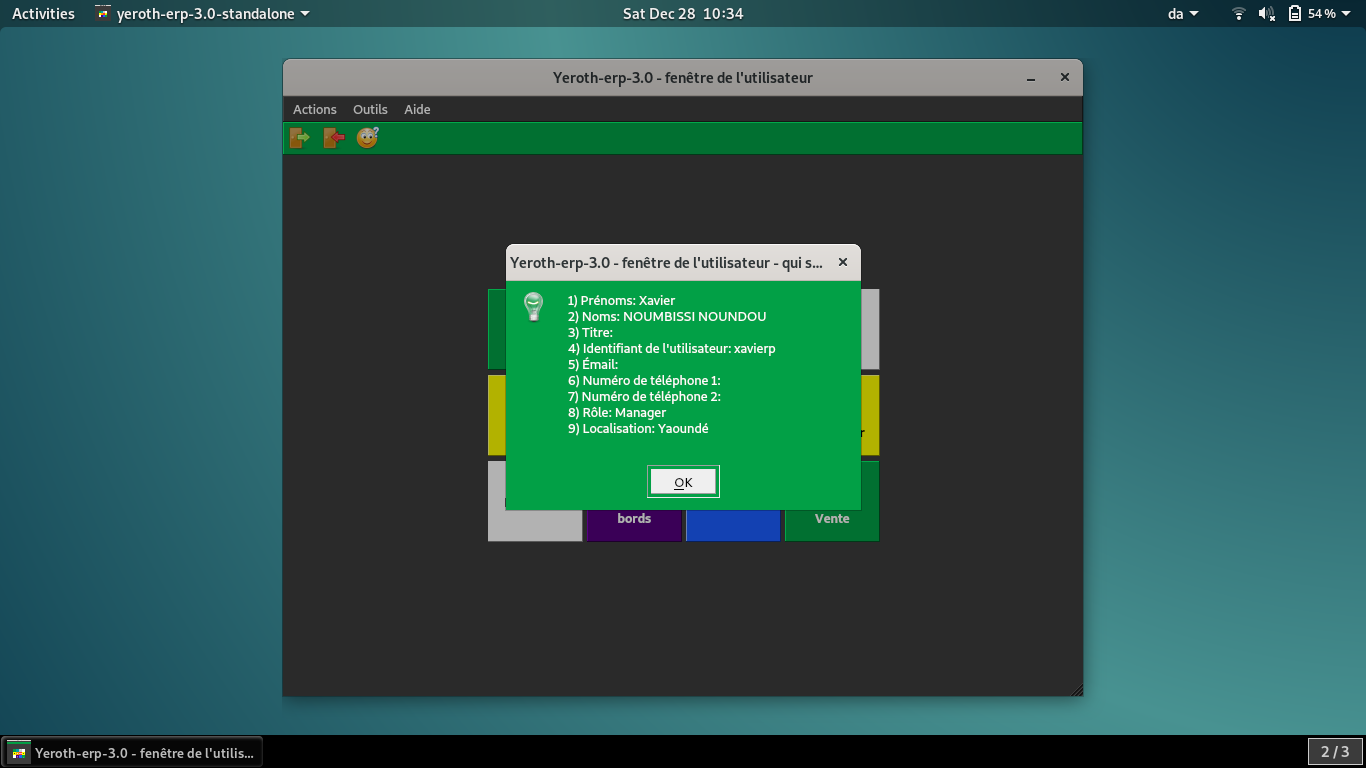
\includegraphics[scale=0.34]{images/yeren-qui-suis-je.png}
	\caption{Un example de la fonctionalit\'e 'Qui suis je ?'.}
	\label{fig:yeren-qui-suis-je}
\end{figure}

La figure~\ref{fig:yeren-qui-suis-je} illustre un example de
la fonctionalit\'e '\textbf{Qui suis je ?}'.

\`A partir de n'importe quelle fen\^etre de \yeroth, cliquez
sur le lien '\textbf{Qui suis je ?}' dans le menu d\'eroulant
'\textbf{Outils}' pour obtenir les informations suivantes
de l'utilisateur avec lequel on s'est enregistr\'e:

\begin{enumerate}[1)]
	\item l'\'email
	\item l'identification de l'utilisateur	
	\item la localisation
	\item les noms	
	\item le num\'ero de t\'el\'ephone 1
	\item le num\'ero de t\'el\'ephone 2	
	\item les pr\'enoms
	\item le r\^ole	
	\item le titre.
\end{enumerate}

%---------------------------------------------------------------

\nxsection{Voir les informations g\'en\'erales de l'entreprise}
\index{voir les informations g\'en\'erales de l'entreprise}

\`A partir de n'importe quelle fen\^etre de \yeroth (except\'e
les fen\^etres de l'administration), cliquez
sur le lien '\textbf{Informations sur l'entreprise}' dans
le menu d\'eroulant '\textbf{Aide}' pour obtenir les
informations suivantes de l'entreprise o\`u \yeroth
est ainsi d\'eploy\'e:

\begin{enumerate}[1)]
	\item l'\'email
	\item l'adresse
	\item la bo\^ite postale
	\item la d\'enomination de l'entreprise
	\item la localisation
	\item le num\'ero de contribuable	
	\item le pays
	\item les secteurs d'activit\'es
	\item le si\`ege social
	\item le t\'el\'ephone
	\item la ville.
\end{enumerate}

La figure~\ref{fig:yeren-informations-generales-entreprise}
illustre un example de la fonctionalit\'e 
'\textbf{Informations sur l'entreprise}'.\\

\begin{figure}[!htbp]
	\centering
	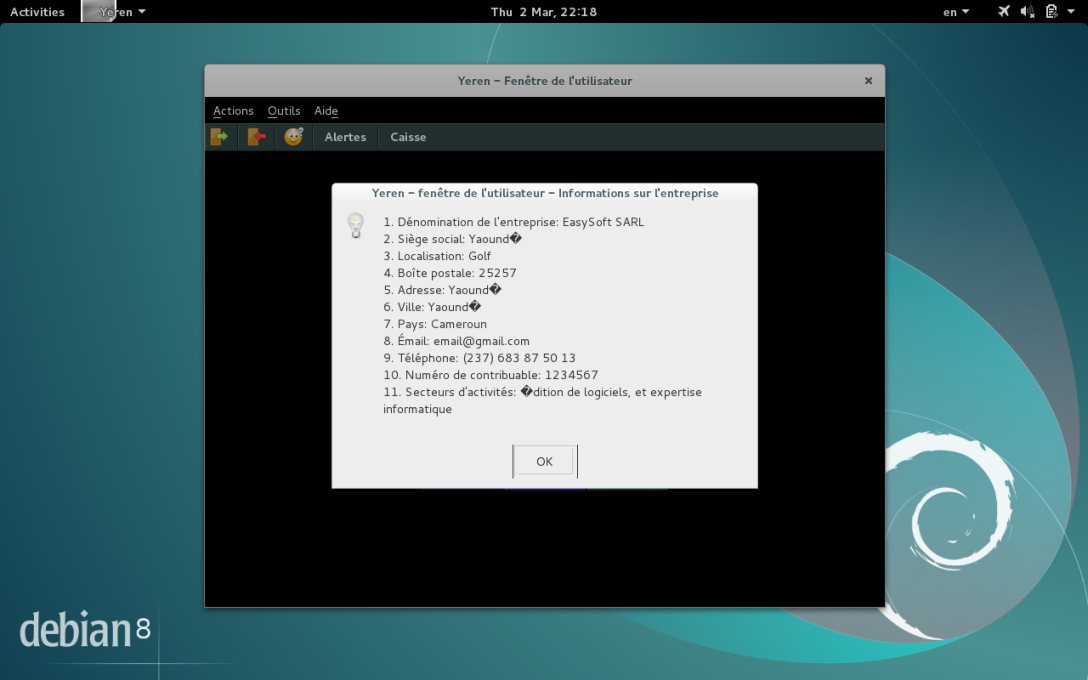
\includegraphics[scale=0.4]{images/yeren-informations-generales-entreprise.png}
	\caption{Un example de la fonctionalit\'e 'Informations sur l'entreprise'.}
	\label{fig:yeren-informations-generales-entreprise}
\end{figure}

%---------------------------------------------------------------

\newpage
\nxsection{Voir le manuel de l'utilisateur au format PDF}
\index{manuel de l'utilisateur au format PDF}

Il suffit de cliquer sur le lien '\textbf{Manuel de l'utilisateur (PDF)}'
qui se trouve dans le menu '\textbf{Aide}' de la fen\^etre
principale de chaque type d'utilisateur de \yeroth:

\begin{enumerate}[1)]
	\item \admin (voir figure~\ref{fig:fenetre-principale-admin})
	\item \caissier (voir figure~\ref{fig:fenetre-principale-caissier})
	\item \magasinier (voir figure~\ref{fig:yeren-fenetre-magasinier})
	\item \manager (voir figure~\ref{fig:yeren-fenetre-patron}).		
\end{enumerate}

%---------------------------------------------------------------

\nxsection{Voir la version de \yeroth que vous utilis\'e}
\index{voir la version de \yeroth que vous utilis\'e}

Il suffit de cliquer sur le lien '\textbf{\`A propos}' qui
se trouve dans le menu '\textbf{Aide}' de n'importe quelle
fen\^etre de \yeroth.

La figure~\ref{fig:yeren-apropos}
illustre un example de la fonctionalit\'e 
'\textbf{\`A propos}'.

\begin{figure}[!htbp]
	\centering
	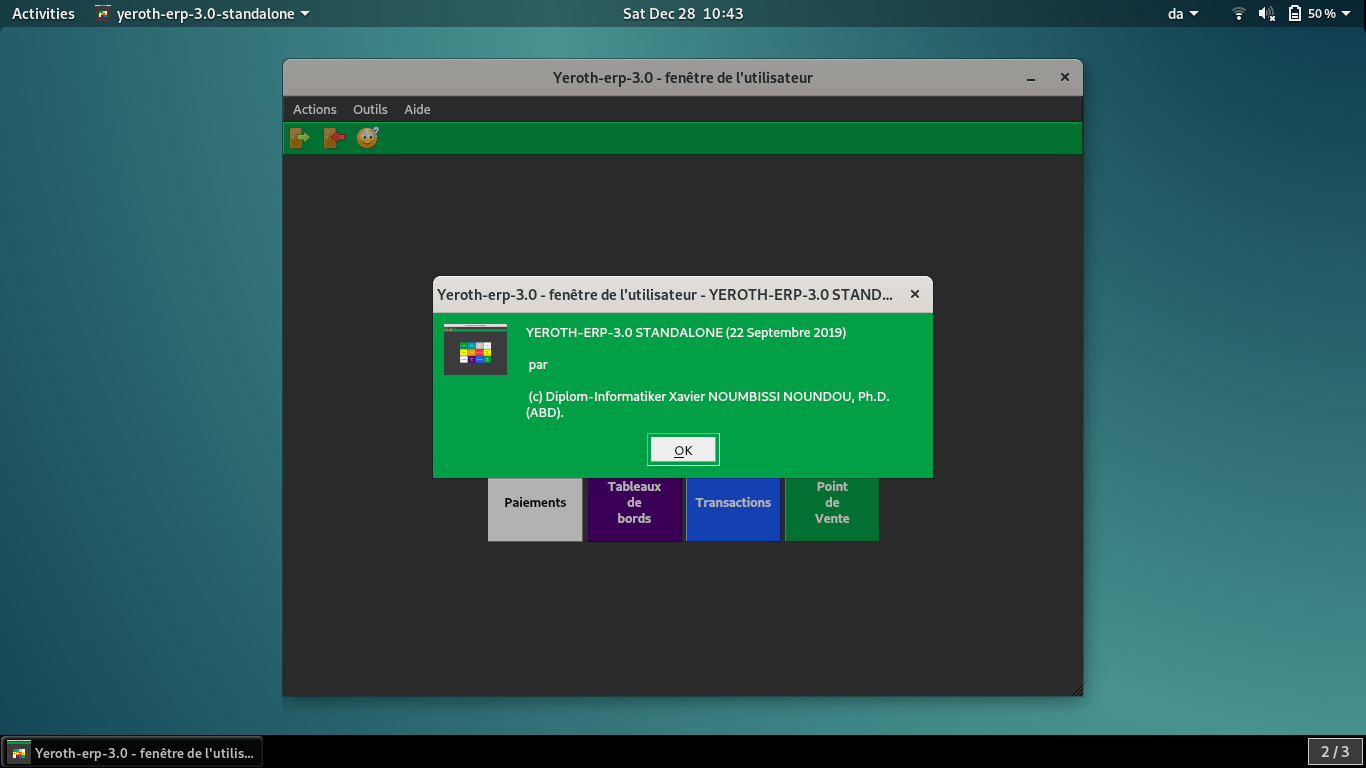
\includegraphics[scale=0.369]{images/yeren-apropos.png}
	\caption{Un example de la fonctionalit\'e '\`A propos'.}
	\label{fig:yeren-apropos}
\end{figure}



\chapter{L'Administration de \yeroth}\label{chap:administration-logiciel}

\utilisateurs: \lienadmin, \lienmanager.\\

\chapintro{Ce chapitre d\'ecrit comment effectu\'e
les t\^aches d'administration (ex: cr\'eer un
nouveau compte pour un utilisateur, etc.).}

\nxsection{Introduction}

\begin{figure}[!htpb]
\centering
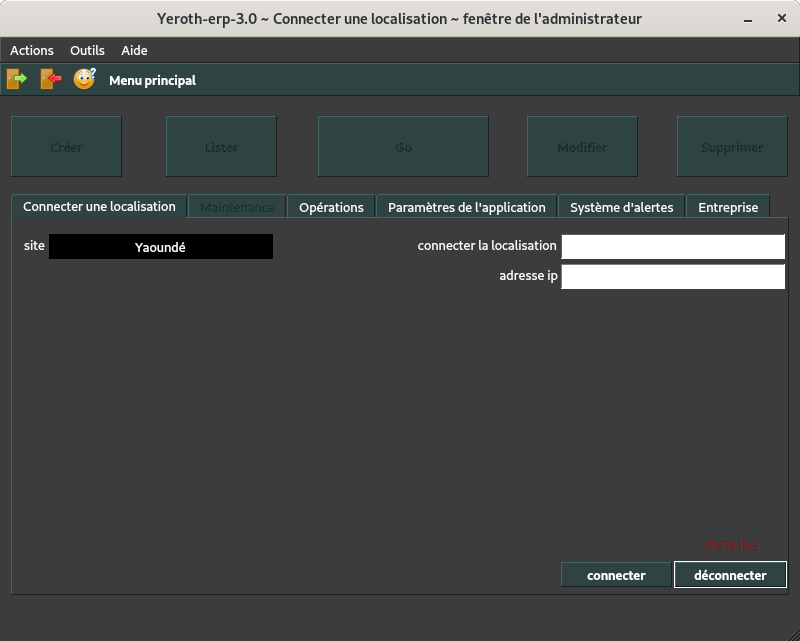
\includegraphics[scale=0.45]{images/yeroth-fenetre-administrateur.png}
\caption{La fen\^etre de l'administrateur.}
\label{fig:fenetre-administrateur}
\end{figure}

La figure~\ref{fig:fenetre-administrateur} illustre la
fen\^etre d'acceuil de l'administration de \yeroth.

On y arrive automatiquement lorsqu'on s'enregistre
\`a \yeroth avec un utilisateur du \role \admin.

Avec un utilisateur du \role \manager, on clique sur le
bouton \bouton{Administration} \`a partir de l'interface
d'acceuil des utilisateurs du \role \manager 
(voir figure~\ref{fig:yeren-fenetre-patron}).

\newpage

%%%%%%%%%%%%%%%%%%%%%%%%%%%%%%%%%%%%%%%%%%%%%%%%%%%%%%%%%%%%%%%%%%%%%%%%%%%%%%%%%

\nxsection{La connection \`a d'autres localisations}
\index{connection \`a d'autres localisations}

La figure~\ref{fig:yeren-admin-connection-autres-db}
illustre l'interface graphique de connection \`a la
base de donn\'ees d'une autre localisation;
cette interface graphique est le $1^{\text{er}}$ onglet
de la fen\^etre de l'administration.

\begin{figure}[!htpb]
	\centering
	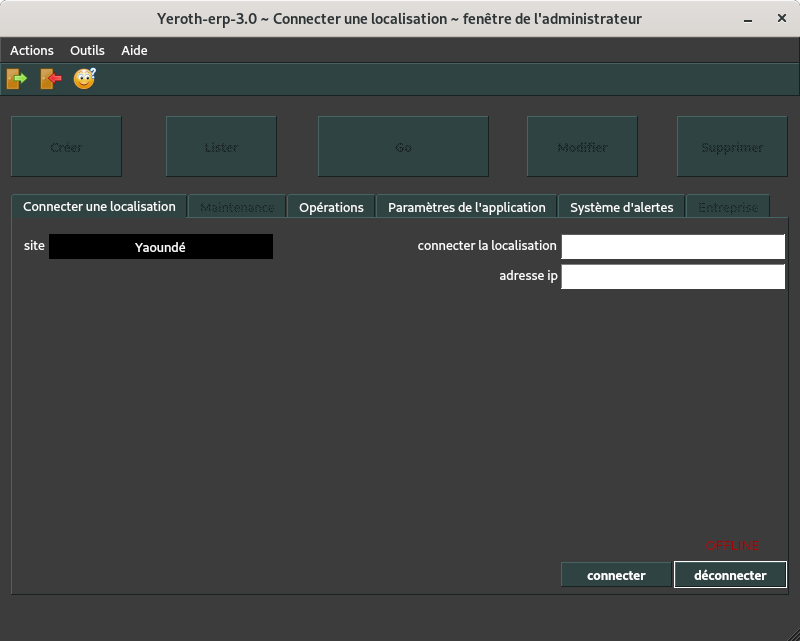
\includegraphics[scale=0.45]{images/yeren-admin-connection-autres-db.png}
	\caption{l'interface graphique de connection de
		\yeroth \`a d'autres localisations.}\label{fig:yeren-admin-connection-autres-db}
\end{figure}

Voici la proc\'edure par laquelle l'utilisateur peut
connecter son installation de \yeroth \`a la base de donn\'ees
d'autres localisations:
\begin{enumerate}[1)]
	\item choisir dans le champs de texte '\textbf{localisation}'
		le nom de localisation \`a laquelle on souhaite
		se connecter. Lorsque cela est fait, l'adresse IP
		de la localisation choisie est automatiquement
		affich\'ee dans le champs de texte '\textbf{adresse IP}'
	
	\item cliquer sur le bouton \bouton{connecter}.
\end{enumerate}

Si la connection est r\'eussie, le mot 
'\textbf{\textcolor{forestgreen}{ONLINE}}' est affich\'e en
couleur verte au dessus du bouton \bouton{connecter}.

%%%%%%%%%%%%%%%%%%%%%%%%%%%%%%%%%%%%%%%%%%%%%%%%%%%%%%%%%%%%%%%%%%%%%%%%%%%%%%%%%

\nxsection{Les param\`etres g\'en\'eraux}
\index{param\`etres g\'en\'eraux}

La figure~\ref{fig:yeren-parametres} illustre l'interface
graphique des param\`etres g\'en\'eraux de \yeroth;
cette interface graphique est le $4^{\text{\`eme}}$
onglet de la fen\^etre de l'administration de \yeroth.

\begin{figure}[!htpb]
	\centering
	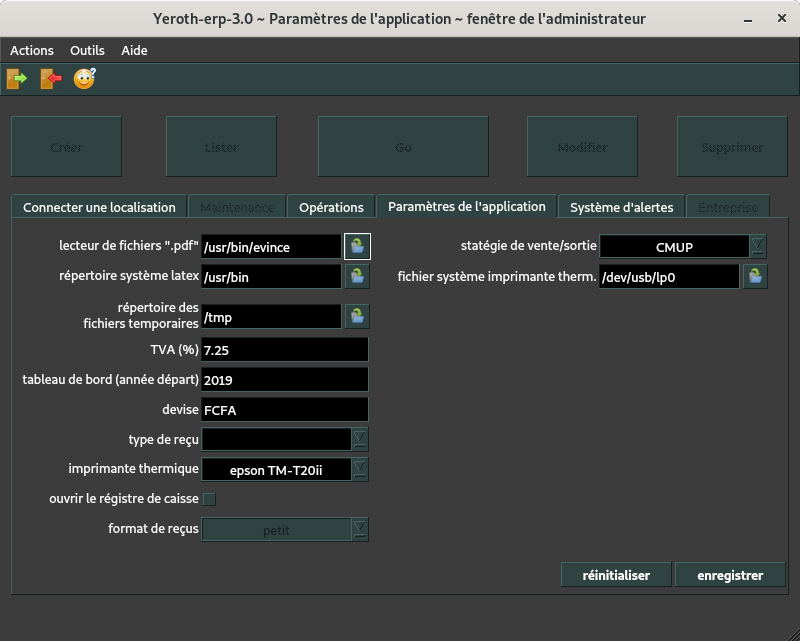
\includegraphics[scale=0.45]{images/yeroth-administration-parametres-generaux.png}
	\caption{l'interface graphique de param\'etrage g\'en\'eral
		de \yeroth.}\label{fig:yeren-parametres}
\end{figure}

Les param\`etres g\'en\'eraux qui peuvent \^etre
modifi\'es sont les suivants:
\begin{enumerate}[1)]
	\item le lecteur des fichiers PDF
	\item le compilateur des fichiers '.tex'
	\item le r\'epertoire des fichiers temporaraires
	\item la taxe sur la valeur ajout\'e
	\item la strat\'egie de vente/sortie des stocks (\cmup, \dpfdpo, \fifo, \lifo)
		\begin{enumerate}[1)]
			\item la s\'election de \cmup pr\'esente tous les
				stocks pr\'esents dans la base de donn\'ees \index{\cmup}
			\item la s\'election \dpfdpo pr\'esente tous les
				stocks selon la strat\'egie ''\textbf{Date of Preemption,
				First Date of Preemption Out}'' \index{\dpfdpo}				
			\item la s\'election de \fifo pr\'esente tous les
				stocks selon la start\'egie ''\textbf{First In, First Out}''
				\index{\fifo}
			\item la s\'election de \lifo pr\'esente tous les
				stocks selon la strat\'egie ''\textbf{Last In, First Out}''
				\index{\lifo}
		\end{enumerate}
	\item le format des fichiers de facturations
	\item l'ann\'ee de d\'epart des rapports lors de la
			g\'en\'eration des chiffres d'affaire.\\
\end{enumerate}

Les strat\'egies de gestion des stocks sont d\'ecrites
dans la section~\ref{sec:strategies-gestion-stocks}.

%%%%%%%%%%%%%%%%%%%%%%%%%%%%%%%%%%%%%%%%%%%%%%%%%%%%%%%%%%%%%%%%%%%%%%%%%%%%%%%%%

\newpage
\nxsection{Les param\`etres du syst\`eme d'alertes}
\index{param\`etres du syst\`eme d'alertes}

La figure~\ref{fig:yeren-admin-alertes-config} illustre
l'interface graphique des param\`etres du syst\`eme d'alertes
de \yeroth; cette interface graphique est le $5^{\text{\`eme}}$
onglet de la fene\^etre de l'administration de \yeroth.

\begin{figure}[!htpb]
	\centering
	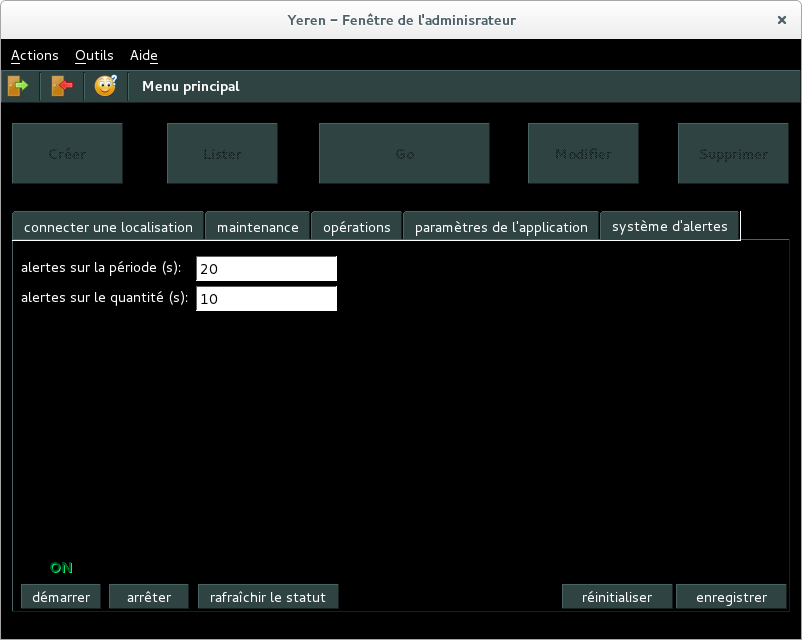
\includegraphics[scale=0.45]{images/yeren-admin-alertes-config.png}
	\caption{l'interface graphique de param\'etrage du
		syst\`eme d'alertes \yeroth.}\label{fig:yeren-admin-alertes-config}
\end{figure}

Le syst\`eme d'alertes est d\'emarr\'e par d\'efaut lors du
d\'emarrage de l'ordinateur. 

Il faut d\'emarrer l'interface graphique de \yeroth en tant
qu'administrateur du syst\`eme d'exploitation afin de
pouvoir stopper le syst\`eme d'alertes lorsqu'il a \'et\'e
d\'emarr\'e lors du d\'emarrage de l'ordinateur.

Les param\`etres du syst\`eme d'alertes qui peuvent \^etre
modifi\'es sont les suivants:
\begin{enumerate}[1)]
	\item \textbf{alertes sur la p\'eriode (s)}: d\'efinit
		l'intervalle de temps (en secondes) apr\`es lequel
		\yeroth visite la base de donn\'ees pour voir
		s'il y'a de nouvelles alertes sur les p\'eriodes de temps
		
	\item \textbf{alertes sur la quantit\'e (s)}: d\'efinit
		l'intervalle de temps (en secondes) apr\`es lequel
		\yeroth visite la base de donn\'ees pour voir
		s'il y'a de nouvelles alertes sur les quantit\'es en stocks.\\
\end{enumerate}

Cette interface graphique permet aussi:
\begin{enumerate}[1)]
	\item de \textbf{d\'emarrer le syst\`eme d'alertes} en pressant
		sur le bouton \bouton{d\'emarrer}. Lorsque le syst\`eme
		d'alertes est en marche, le mot anglais
		'\textbf{\textcolor{forestgreen}{ON}}' est
		affich\'e en vert au dessus du boutton \bouton{d\'emarrer}.
		
	\item \textbf{d'arr\^eter le syst\`eme d'alertes} en pressant
		sur le bouton \bouton{arr\^eter}. Lorsque le syst\`eme
		d'alertes n'est pas en marche, le mot anglais
		'\textbf{\textcolor{firebrickred}{OFF}}' est
		affich\'e en couleur rouge au dessus du boutton \bouton{arr\^eter}.
		
		Cette action n\'ecessite que l'utilisateur est d\'emarr\'e
		\yeroth en tant qu'administrateur du syst\`eme d'exploitation.
		
	\item \textbf{d'actualiser le statut} dans lequel se trouve
		le syst\`eme d'alertes en pressant sur le bouton
		\bouton{rafra\^ichir le statut}.		
\end{enumerate}
%-----------------------------------------------------------

\newpage
\nxsection{Les Alertes}\label{sec:administration-alertes}
\index{les alertes}

\nxsubsection{Afficher les d\'etails d'une alerte}
\index{afficher les d\'etails d'une alerte}

La figure~\ref{fig:admin-alertes-afficher-details} illustre
l'interface graphique de \yeroth qui affiche les d\'etails
d'une alerte.\\

\begin{figure}[!htpb]
	\centering
	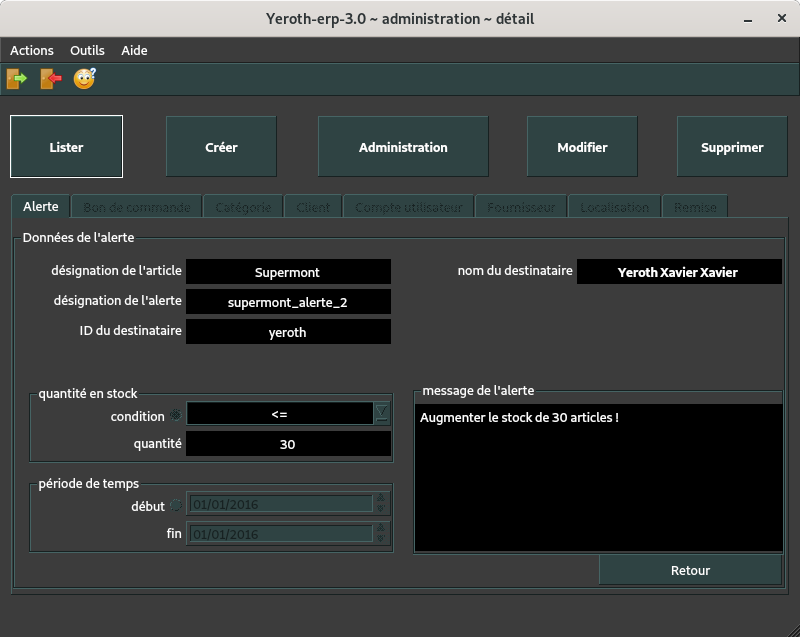
\includegraphics[scale=0.45]{images/alerte-afficher-details.png}
	\caption{Une interface graphique de \yeroth qui affiche les d\'etails
	d'une alerte.}\label{fig:admin-alertes-afficher-details}
\end{figure}

\procparagraph{Proc\'edure pour afficher les d\'etails d'une alerte}
\begin{enumerate}[1)]
	\item \`A partir de l'interface graphique de l'acceuil de
		l'administration (voir figure~\ref{fig:fenetre-administrateur}),
		on clique sur l'onglet intitul\'e \textbf{op\'erations}. 
		
	\item Choisir '\textbf{lister}' dans le '\emph{combo box
		op\'erations}'.
		
	\item Choisir '\textbf{une alerte}' dans le '\emph{combo box
		sujets}'. Vous \^etes automatiquement conduit \`a la fen\^etre
		illustr\'ee par la figure~\ref{fig:admin-alertes-lister}.
		
	\item S\'electionner l'alerte dont vous souhaitez afficher
		les d\'etails dans la liste des alertes affich\'ee.
		
	\item Cliquer sur le bouton \bouton{Afficher}. Les d\'etails
		sur le stock sont affich\'es dans une nouvelle fen\^etre.
\end{enumerate}

%%%%%%%%%%%%%%%%%%%%%%%%%%%%%%%%%%%%%%%%%%%%%%%%%%%%%%%%%%%%%%%%%%%%%%%%%%%%%%%%%

\newpage
\nxsubsection{Cr\'eer une alerte}\label{sec:administration-alertes-creer}
\index{cr\'eer une alerte}

La figure~\ref{fig:admin-alertes-creer} illustre l'interface
graphique de \yeroth pour cr\'eer une alerte.\\

\begin{figure}[!htpb]
	\centering
	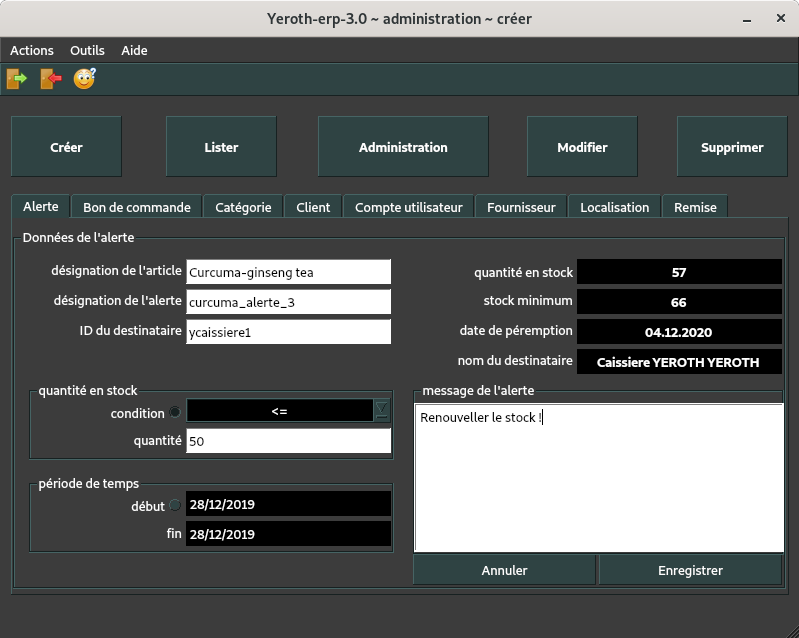
\includegraphics[scale=0.45]{images/alerte-creer.png}
	\caption{L'interface graphique pour cr\'eer des alertes.}
	\label{fig:admin-alertes-creer}
\end{figure}

\procparagraph{Proc\'edure pour cr\'eer une alerte}
Consulter les sections~\ref{sec:alerte-quantite-stock}
et~\ref{sec:alerte-periode-temps} pour savoir comment
cr\'eer respectivement des alertes sur la quantit\'e en
stock et des alertes sur la p\'eriode de temps.

%%%%%%%%%%%%%%%%%%%%%%%%%%%%%%%%%%%%%%%%%%%%%%%%%%%%%%%%%%%%%%%%%%%%%%%%%%%%%%%%%

\newpage
\nxsubsection{Lister les alertes}\label{sec:administration-alertes-lister}
\index{lister les alertes}

La figure~\ref{fig:admin-alertes-lister} illustre l'interface
graphique de \yeroth qui liste les alertes.\\

\begin{figure}[!htpb]
	\centering
	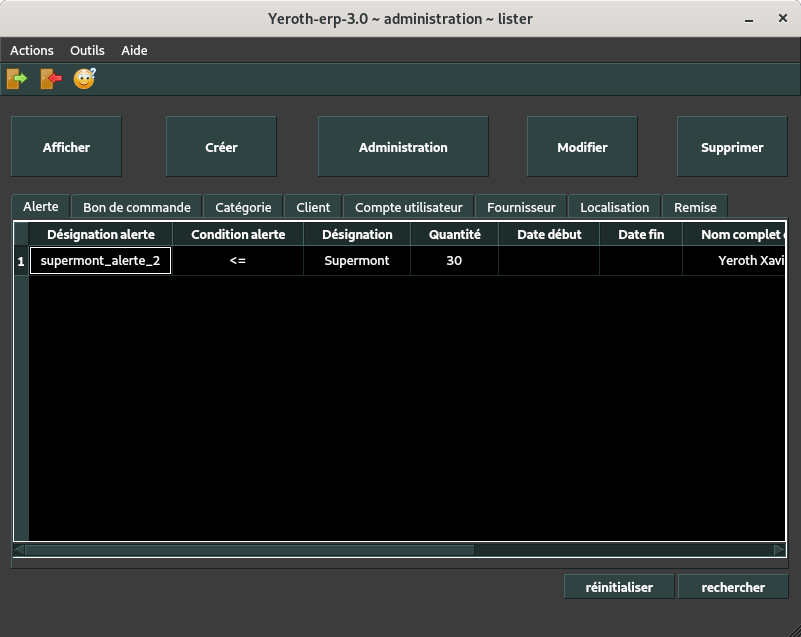
\includegraphics[scale=0.45]{images/alerte-lister.png}
	\caption{L'interface graphique qui liste les alertes.}
	\label{fig:admin-alertes-lister}
\end{figure}

\procparagraph{Proc\'edure pour lister les alertes}
\begin{enumerate}[1)]
	\item \`A partir de l'interface graphique de l'acceuil de
		l'administration (voir la figure~\ref{fig:fenetre-administrateur}),
		on clique sur l'onglet intitul\'e \textbf{op\'erations}. 
		
	\item Choisir '\textbf{lister}' dans le '\emph{combo box
		op\'erations}'.
		
	\item Choisir '\textbf{une alerte}' dans le '\emph{combo box
		sujets}'. Vous \^etes automatiquement conduit \`a la fen\^etre
		qui liste les alertes (voir la figure~\ref{fig:admin-alertes-lister}).
\end{enumerate}

%%%%%%%%%%%%%%%%%%%%%%%%%%%%%%%%%%%%%%%%%%%%%%%%%%%%%%%%%%%%%%%%%%%%%%%%%%%%%%%%%

\newpage
\nxsubsection{Modifier les d\'etails d'une alerte}
\index{modifier les d\'etails d'une alerte}

La figure~\ref{fig:admin-alertes-modifier} illustre
l'interface graphique de \yeroth pour modifier les
d\'etails d'une alerte.\\

\begin{figure}[!htpb]
	\centering
	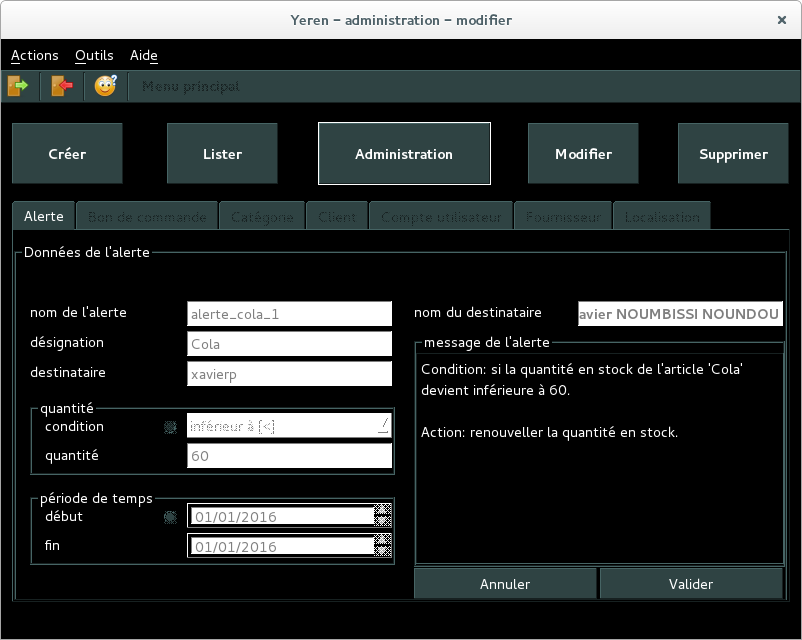
\includegraphics[scale=0.45]{images/alerte-modifier.png}
	\caption{L'interface graphique pour modifier les d'\'etails
	d'une alerte.}\label{fig:admin-alertes-modifier}
\end{figure}

\procparagraph{Proc\'edure pour modifier les d\'etails d'une alerte}
\begin{enumerate}[1)]
	\item \`A partir de l'interface graphique de l'acceuil de
		l'administration (voir figure~\ref{fig:fenetre-administrateur}),
		on clique sur l'onglet intitul\'e \textbf{op\'erations}. 
		
	\item Choisir '\textbf{lister}' dans le '\emph{combo box
		op\'erations}'.
		
	\item Choisir '\textbf{une alerte}' dans le '\emph{combo box
		sujets}'. Vous \^etes automatiquement conduit \`a la fen\^etre
		illustr\'ee par la figure~\ref{fig:admin-alertes-lister}.
		
	\item S\'electionner l'alerte dont vous souhaitez modifier
		les d\'etails dans la liste des alertes affich\'ee.
		
	\item Cliquer sur le bouton \bouton{Modifier}. Les d\'etails
		sur le stock sont affich\'es dans une nouvelle fen\^etre.
		
	\item Faites les modifications que vous souhaitez. Pour
		les alertes, seul le message d'alerte peut \^etre
		modifi\'e.
		
	\item Cliquer sur le bouton \bouton{valider} pour valider
		les modifications faites.
\end{enumerate}

%%%%%%%%%%%%%%%%%%%%%%%%%%%%%%%%%%%%%%%%%%%%%%%%%%%%%%%%%%%%%%%%%%%%%%%%%%%%%%%%%

\newpage
\nxsubsection{Supprimer une alerte}
\index{supprimer une alerte}

La figure~\ref{fig:admin-alertes-supprimer} illustre l'interface
graphique de \yeroth pour supprimer une alerte.\\

\begin{figure}[!htpb]
	\centering
	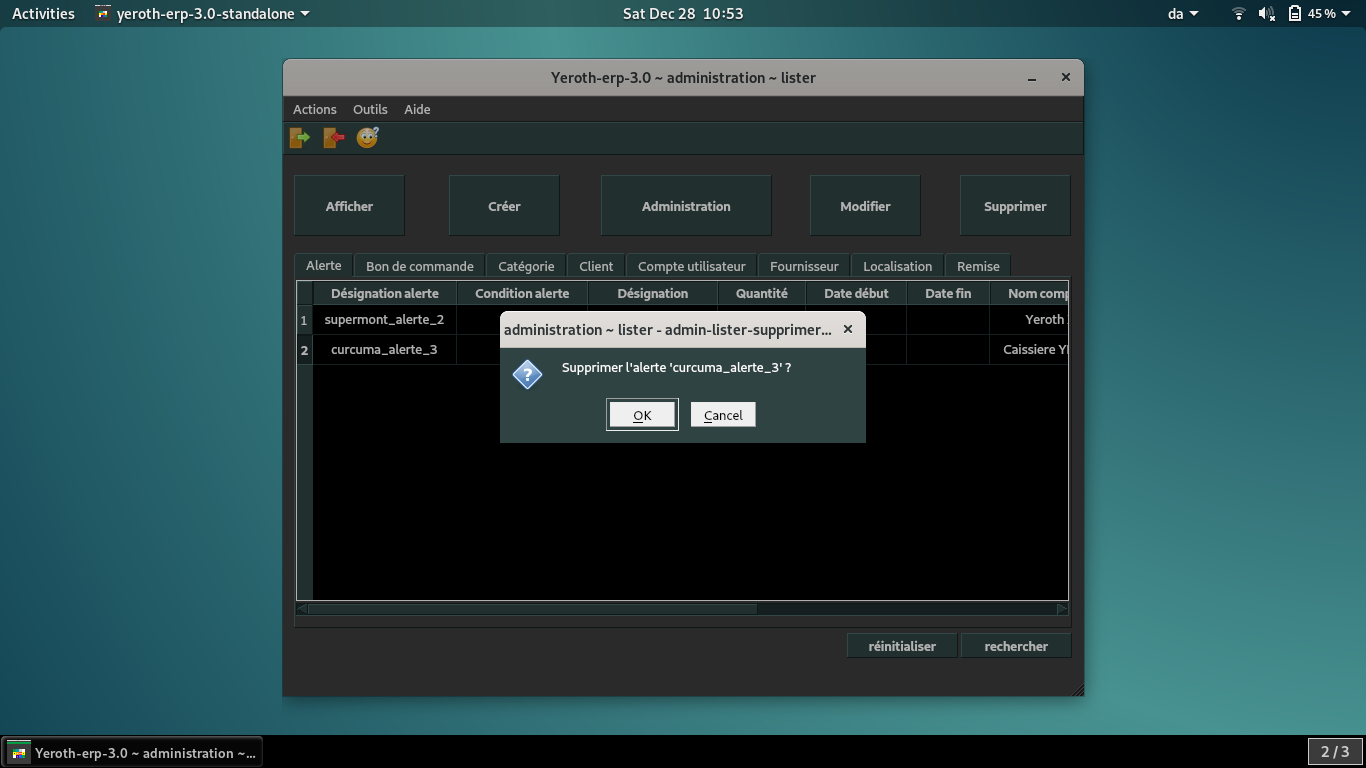
\includegraphics[scale=0.35]{images/alerte-supprimer.png}
	\caption{L'interface graphique pour supprimer des alertes.}
	\label{fig:admin-alertes-supprimer}
\end{figure}

\procparagraph{Proc\'edure pour supprimer une alerte}
\begin{enumerate}[1)]
	\item \`A partir de l'interface graphique de l'acceuil de
		l'administration (voir figure~\ref{fig:fenetre-administrateur}),
		on clique sur l'onglet intitul\'e \textbf{op\'erations}. 
		
	\item Choisir '\textbf{supprimer}' dans le '\emph{combo box
		op\'erations}'.
		
	\item Choisir '\textbf{une alerte}' dans le '\emph{combo box
		sujets}'. Vous \^etes automatiquement conduit \`a la fen\^etre
		illustr\'ee par la figure~\ref{fig:admin-alertes-lister}.
		
	\item S\'electionner l'alerte \`a supprimer dans la liste
		des alertes affich\'ee.
		
	\item Cliquer sur le bouton \bouton{Supprimer}. La question
		est ensuite pos\'ee si vous confirmer votre choix.
		Cliquer sur le \bouton{OK} pour confirmer votre choix.
\end{enumerate}

\newpage

%-----------------------------------------------------------

\nxsection{Les Cat\'egories d'Articles}
\index{les cat\'egories d'articles}

\nxsubsection{Afficher les d\'etails d'une cat\'egorie d'articles}
\index{afficher les d\'etails d'une cat\'egorie d'articles}
\index{d\'etails d'une cat\'egorie d'articles}

\begin{figure}[!htpb]
	\centering
	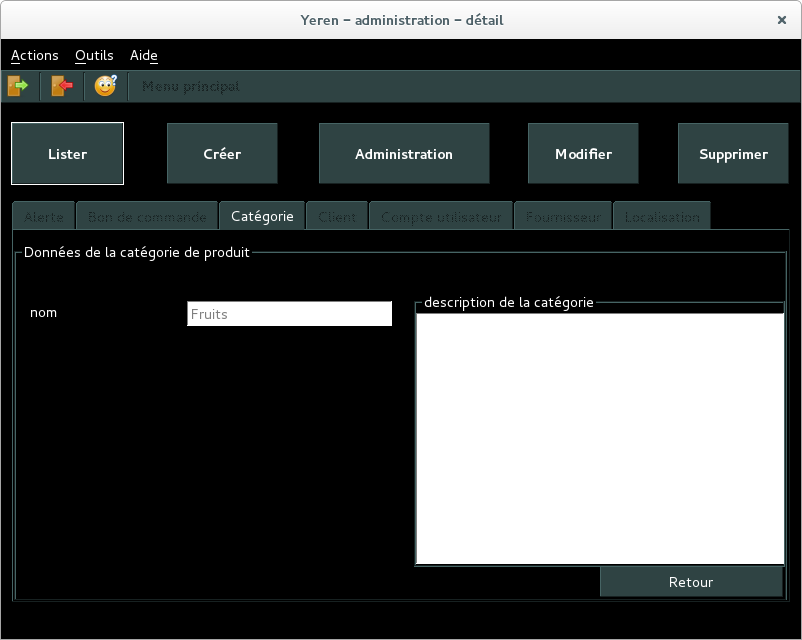
\includegraphics[scale=0.45]{images/categorie-articles-afficher-details.png}
	\caption{L'interface graphique pour afficher les d\'etails d'une
			cat\'egorie d'articles.}
	\label{fig:admin-categories-articles-afficher-details}
\end{figure}

La figure~\ref{fig:admin-categories-articles-afficher-details}
illustre l'interface graphique de \yeren qui affiche
les d\'etails d'une cat\'egorie d'articles.

\procparagraph{Proc\'edure pour afficher les d\'etails
	d'une cat\'egorie d'articles}
\begin{enumerate}[1)]
	\item \`A partir de l'interface graphique de l'acceuil de
		l'administration (voir figure~\ref{fig:fenetre-administrateur}),
		on clique sur l'onglet intitul\'e \textbf{op\'erations}. 
		
	\item Choisir '\textbf{lister}' dans le '\emph{combo box
		op\'erations}'.
		
	\item Choisir '\textbf{une cat\'egorie d'articles}' dans le
		'\emph{combo box objets}'. Vous \^etes automatiquement
		conduit \`a la fen\^etre illustr\'ee par la
		figure~\ref{fig:admin-categories-articles-lister}.
		
	\item S\'electionner la cat\'egorie d'articles dont vous
		souhaitez afficher les d\'etails.
		
	\item Cliquer sur le bouton \bouton{Afficher}. Les d\'etails
		sur la cat\'egorie d'articles sont affich\'es dans une
		nouvelle fen\^etre.
\end{enumerate}

%%%%%%%%%%%%%%%%%%%%%%%%%%%%%%%%%%%%%%%%%%%%%%%%%%%%%%%%%%%%%%%%%%%%%%%%%%%%%%%%%

\newpage
\nxsubsection{Cr\'eer une cat\'egorie d'articles}
\index{cr\'eer une cat\'egorie d'articles}

\begin{figure}[!htpb]
	\centering
	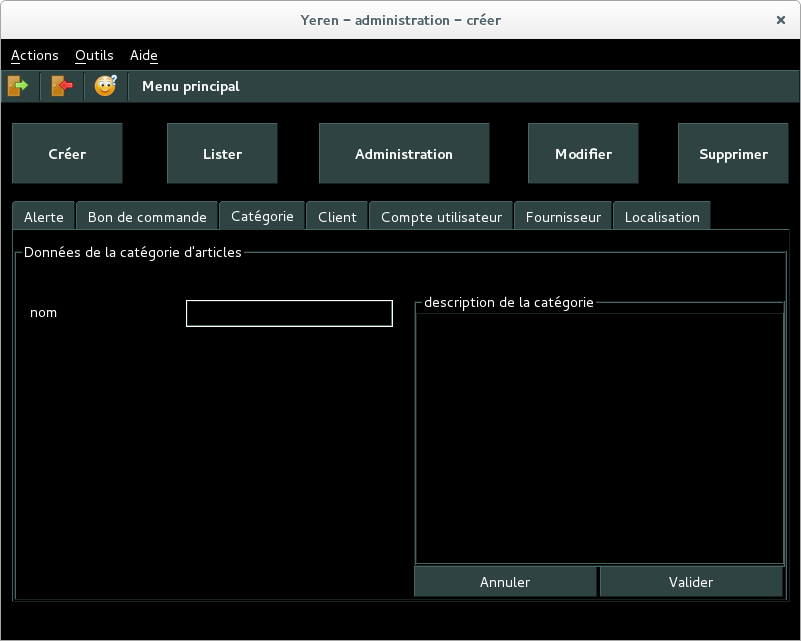
\includegraphics[scale=0.45]{images/categorie-articles-creer.png}
	\caption{L'interface graphique pour cr\'eer une cat\'egorie d'articles.}
	\label{fig:admin-categories-articles-creer}
\end{figure}

La figure~\ref{fig:admin-categories-articles-creer} illustre
l'interface graphique de \yeren pour cr\'eer une nouvelle
cat\'egorie d'articles.

\procparagraph{Proc\'edure pour cr\'eer une cat\'egorie d'articles}
\begin{enumerate}[1)]
	\item \`A partir de l'interface graphique de l'acceuil de
		l'administration (voir figure~\ref{fig:fenetre-administrateur}),
		on clique sur l'onglet intitul\'e \textbf{op\'erations}. 
		
	\item Choisir '\textbf{cr\'eer}' dans le '\emph{combo box
		op\'erations}'.
		
	\item Choisir '\textbf{une cat\'egorie d'articles}' dans
		le '\emph{combo box objets}'. Vous \^etes automatiquement
		conduit \`a la fen\^etre illustr\'ee par la
		figure~\ref{fig:admin-categories-articles-creer}.
		
	\item Saisissez la d\'esignation de la nouvelle cat\'egorie
		d'articles \`a cr\'eer dans le champs de texte
		'\textbf{d\'esignation}'.

	\item Si vous le souhaitez, saisisser un texte qui d\'ecrit
		cette nouvelle cat\'egorie d'articles dans le champs de
		texte '\textbf{description de la cat\'egorie}'.
		
	\item Cliquer sur le bouton \bouton{Valider} pour
		valider votre travail.		
\end{enumerate}

%%%%%%%%%%%%%%%%%%%%%%%%%%%%%%%%%%%%%%%%%%%%%%%%%%%%%%%%%%%%%%%%%%%%%%%%%%%%%%%%%

\newpage
\nxsubsection{Lister les cat\'egories d'articles}\label{sec:administration-categorie-lister}
\index{lister les cat\'egories d'articles}

\begin{figure}[!htpb]
	\centering
	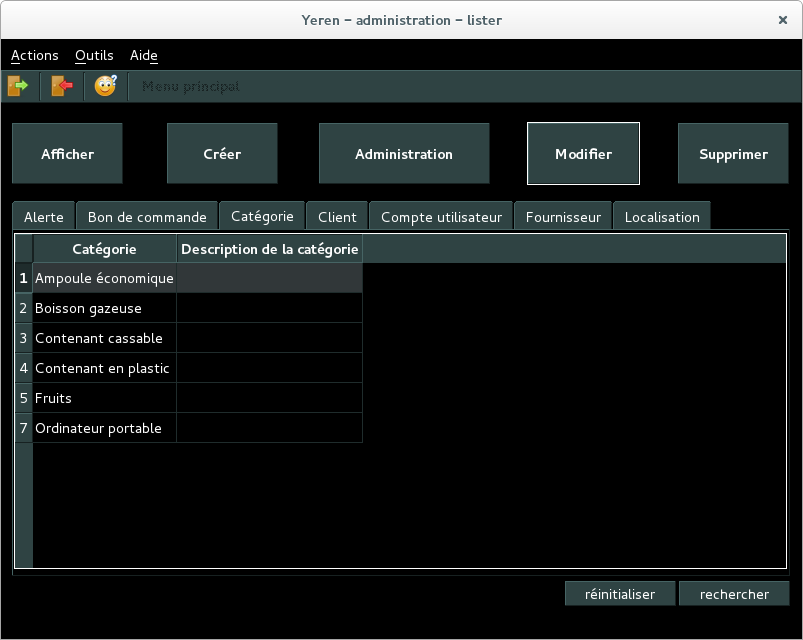
\includegraphics[scale=0.45]{images/categorie-articles-lister.png}
	\caption{L'interface graphique qui liste les cat\'egories d'articles.}
	\label{fig:admin-categories-articles-lister}
\end{figure}

La figure~\ref{fig:admin-categories-articles-lister} illustre
l'interface graphique de \yeren qui liste les cat\'egories
d'articles.

\procparagraph{Proc\'edure pour lister les cat\'egories d'articles}
\begin{enumerate}[1)]
	\item \`A partir de l'interface graphique de l'acceuil de
		l'administration (voir figure~\ref{fig:fenetre-administrateur}),
		on clique sur l'onglet intitul\'e \textbf{op\'erations}. 
		
	\item Choisir '\textbf{lister}' dans le '\emph{combo box
		op\'erations}'.
		
	\item Choisir '\textbf{une cat\'egorie d'articles}' dans
		le '\emph{combo box objets}'. Vous \^etes automatiquement
		conduit \`a la fen\^etre qui liste les cat\'egories
		d'articles (figure~\ref{fig:admin-categories-articles-lister}).
\end{enumerate}

%%%%%%%%%%%%%%%%%%%%%%%%%%%%%%%%%%%%%%%%%%%%%%%%%%%%%%%%%%%%%%%%%%%%%%%%%%%%%%%%%

\newpage
\nxsubsection{Modifier les d\'etails d'une cat\'egorie d'articles}
\index{modifier les d\'etails d'une cat\'egorie d'articles}

\begin{figure}[!htpb]
	\centering
	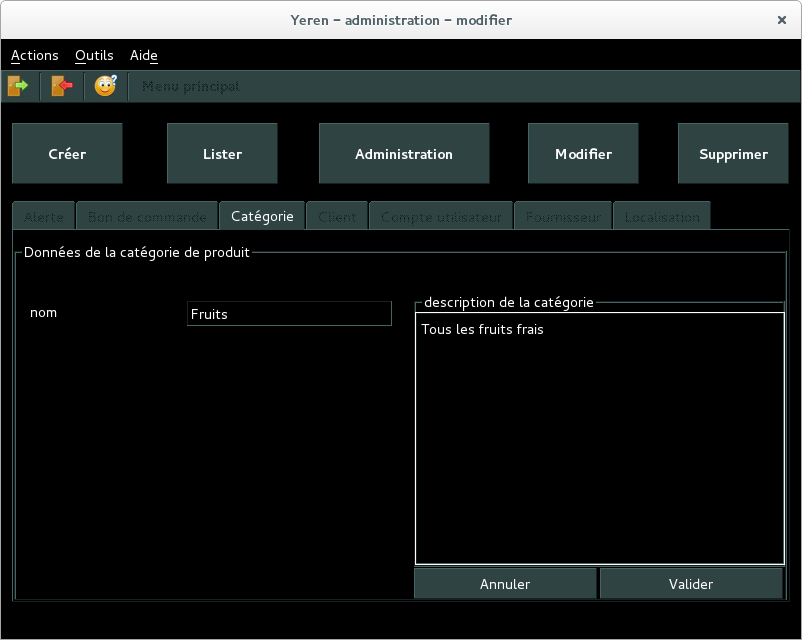
\includegraphics[scale=0.45]{images/categorie-articles-modifier.png}
	\caption{L'interface graphique pour modifier les d'\'etails
			d'une cat\'egorie d'articles.}
	\label{fig:admin-categories-articles-modifier}
\end{figure}

La figure~\ref{fig:admin-categories-articles-modifier}
illustre l'interface graphique de \yeren pour modifier
les d\'etails d'une cat\'egorie d'articles.

\procparagraph{Proc\'edure pour modifier les d\'etails
	d'une cat\'egorie d'articles}
\begin{enumerate}[1)]
	\item \`A partir de l'interface graphique de l'acceuil de
		l'administration (voir figure~\ref{fig:fenetre-administrateur}),
		on clique sur l'onglet intitul\'e \textbf{op\'erations}. 
		
	\item Choisir '\textbf{lister}' dans le '\emph{combo box
		op\'erations}'.
		
	\item Choisir '\textbf{cat\'egorie d'articles}' dans le
		'\emph{combo box objets}'. Vous \^etes automatiquement
		conduit \`a la fen\^etre illustr\'ee par la
		figure~\ref{fig:admin-categories-articles-lister}.
		
	\item S\'electionner l'alerte dont vous souhaitez modifier
		les d\'etails dans la liste	des d\'esignations des
		cat\'egories d'articles affich\'ee.
		
	\item Cliquer sur le bouton \bouton{Modifier}. Les d\'etails
		sur le stock sont affich\'es dans une nouvelle fen\^etre.
		
	\item Faites les modifications que vous souhaitez. Pour
		les alertes, seul le message d'alerte peut \^etre
		modifi\'e.
		
	\item Cliquer sur le bouton \bouton{valider} pour valider
		les modifications faites.
\end{enumerate}

%%%%%%%%%%%%%%%%%%%%%%%%%%%%%%%%%%%%%%%%%%%%%%%%%%%%%%%%%%%%%%%%%%%%%%%%%%%%%%%%%

\newpage
\nxsubsection{Supprimer une cat\'egorie d'article}
\index{supprimer une cat\'egorie d'article}

\begin{figure}[!htpb]
	\centering
	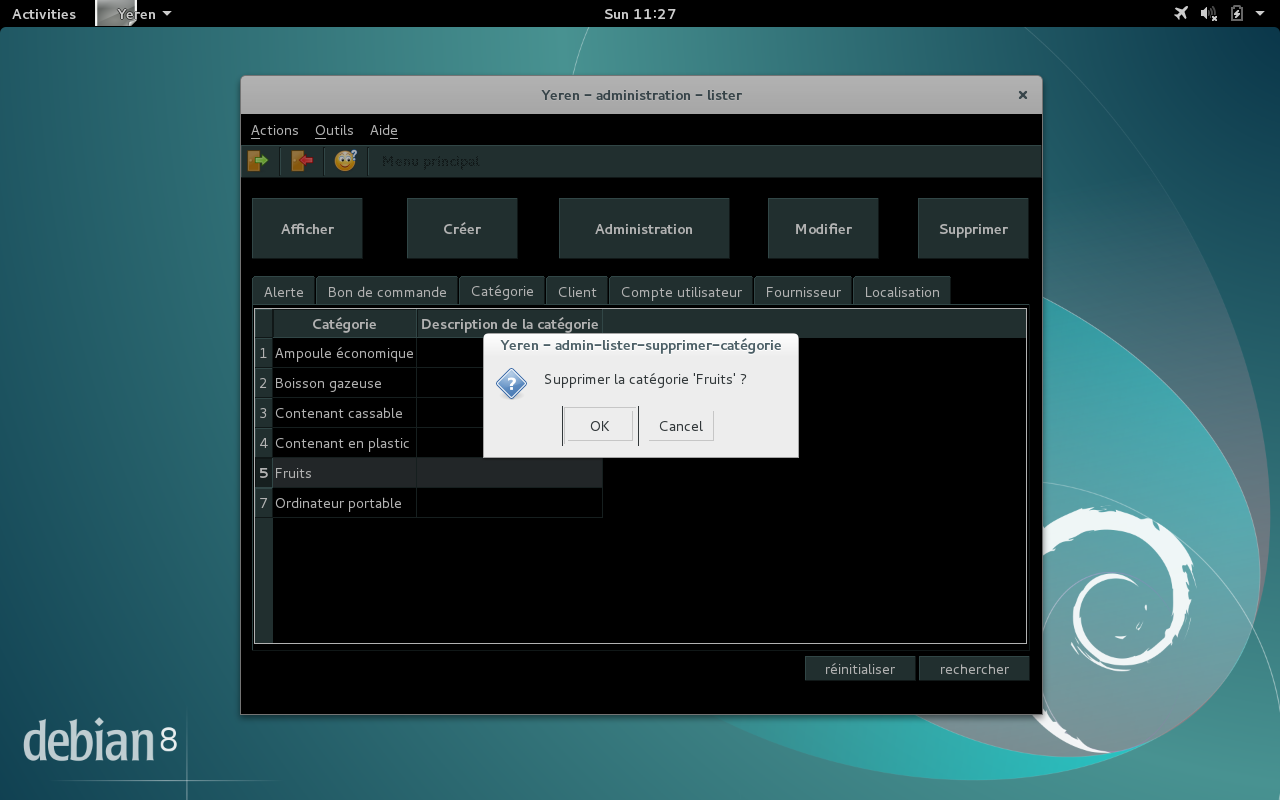
\includegraphics[scale=0.39]{images/categorie-articles-supprimer.png}
	\caption{L'interface graphique pour supprimer une cat\'egorie d'articles.}
	\label{fig:admin-categories-articles-supprimer}
\end{figure}

La figure~\ref{fig:admin-categories-articles-supprimer} illustre
l'interface graphique de \yeren pour supprimer une
cat\'egorie d'articles.

\procparagraph{Proc\'edure pour supprimer une cat\'egorie d'articles}
\begin{enumerate}[1)]
	\item \`A partir de l'interface graphique de l'acceuil de
		l'administration (voir figure~\ref{fig:fenetre-administrateur}),
		on clique sur l'onglet intitul\'e \textbf{op\'erations}. 
		
	\item Choisir '\textbf{supprimer}' dans le '\emph{combo box
		op\'erations}'.
		
	\item Choisir '\textbf{une cat\'egorie d'articles}' dans le
		'\emph{combo box objets}'. Vous \^etes automatiquement
		conduit \`a la fen\^etre illustr\'ee par la
		figure~\ref{fig:admin-categories-articles-lister}.
		
	\item S\'electionner l'alerte \`a supprimer dans la liste
		des d\'esignations des cat\'egories d'articles affich\'ee.
		
	\item Cliquer sur le bouton \bouton{Supprimer}. La question
		est ensuite pos\'ee si vous confirmer votre choix.
		Cliquer sur le \bouton{OK} pour confirmer votre choix.
\end{enumerate}

\newpage

%-----------------------------------------------------------

\nxsection{Les Comptes Clients}
\index{les comptes clients}

\nxsubsection{Afficher les d\'etails d'un compte client}
\index{afficher les d\'etails d'un compte client}

\begin{figure}[!htpb]
	\centering
	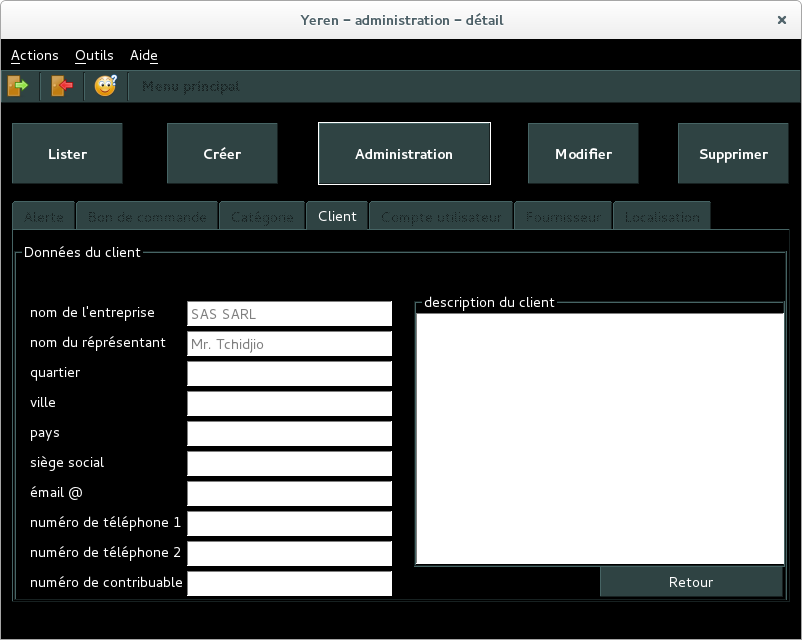
\includegraphics[scale=0.45]{images/compte-client-afficher-details.png}
	\caption{L'interface graphique pour afficher les d\'etails d'un compte client.}
	\label{fig:admin-compte-client-afficher-details}
\end{figure}

La figure~\ref{fig:admin-compte-client-afficher-details}
illustre l'interface graphique de \yeren qui affiche les
d\'etails d'un compte client.

\procparagraph{Proc\'edure pour afficher les d\'etails d'un compte client}
\begin{enumerate}[1)]
	\item \`A partir de l'interface graphique de l'acceuil de
		l'administration (voir figure~\ref{fig:fenetre-administrateur}),
		on clique sur l'onglet intitul\'e \textbf{op\'erations}. 
		
	\item Choisir '\textbf{lister}' dans le '\emph{combo box
		op\'erations}'.
		
	\item Choisir '\textbf{un compte client}' dans le '\emph{combo box
		sujets}'. Vous \^etes automatiquement conduit \`a la fen\^etre
		illustr\'ee par la figure~\ref{fig:admin-comptes-clients-lister}.
		
	\item S\'electionner le compte client dont vous souhaitez afficher
		les d\'etails dans la liste des comptes clients affich\'ee.
		
	\item Cliquer sur le bouton \bouton{Afficher}. Les d\'etails
		du compte client sont affich\'es dans une nouvelle fen\^etre.
\end{enumerate}

%------------------------------------------------------------------------------

\newpage
\nxsubsection{Cr\'eer un compte client}\label{sec:administration-comptes-clients-lister}
\index{cr\'eer un compte client}

\begin{figure}[!htpb]
	\centering
	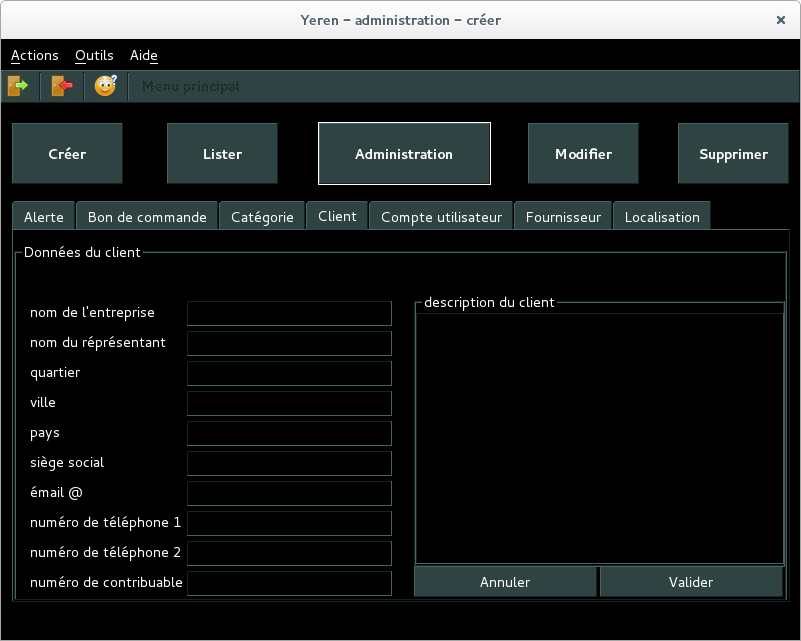
\includegraphics[scale=0.45]{images/compte-client-creer.png}
	\caption{L'interface graphique pour cr\'eer un compte client.}
	\label{fig:admin-comptes-clients-creer}
\end{figure}

La figure~\ref{fig:admin-comptes-clients-creer} illustre
l'interface graphique de \yeren pour cr\'eer un nouveau
compte client.

\procparagraph{Proc\'edure pour cr\'eer un compte client}
\begin{enumerate}[1)]
	\item \`A partir de l'interface graphique de l'acceuil de
		l'administration (voir figure~\ref{fig:fenetre-administrateur}),
		on clique sur l'onglet intitul\'e \textbf{op\'erations}. 
		
	\item Choisir '\textbf{cr\'eer}' dans le '\emph{combo box
		op\'erations}'.
		
	\item Choisir '\textbf{un compte client}' dans
		le '\emph{combo box objets}'. Vous \^etes automatiquement
		conduit \`a la fen\^etre illustr\'ee par la
		figure~\ref{fig:admin-comptes-clients-creer}.
		
	\item Saisissez les informations requises dans les champs de texte
		suivants:
		\begin{enumerate}[1)]
			\item nom de l'entreprise \obligatoire
			\item nom du r\'epr\'esentant \obligatoire
			\item quartier
			\item ville 
			\item pays
			\item si\`ege social 
			\item \'email@ 
			\item num\'ero de t\'el\'ephone 1 
			\item num\'ero de t\'el\'ephone 2
			\item num\'ero de contribuable 
			\item description du client.			
		\end{enumerate}
		
	\item Cliquer sur le bouton \bouton{Valider} pour
		valider votre travail.		
\end{enumerate}

%------------------------------------------------------------------------------

\newpage
\nxsubsection{Lister les comptes clients}\label{sec:administration-comptes-clients-lister}
\index{lister les comptes clients}

\begin{figure}[!htpb]
	\centering
	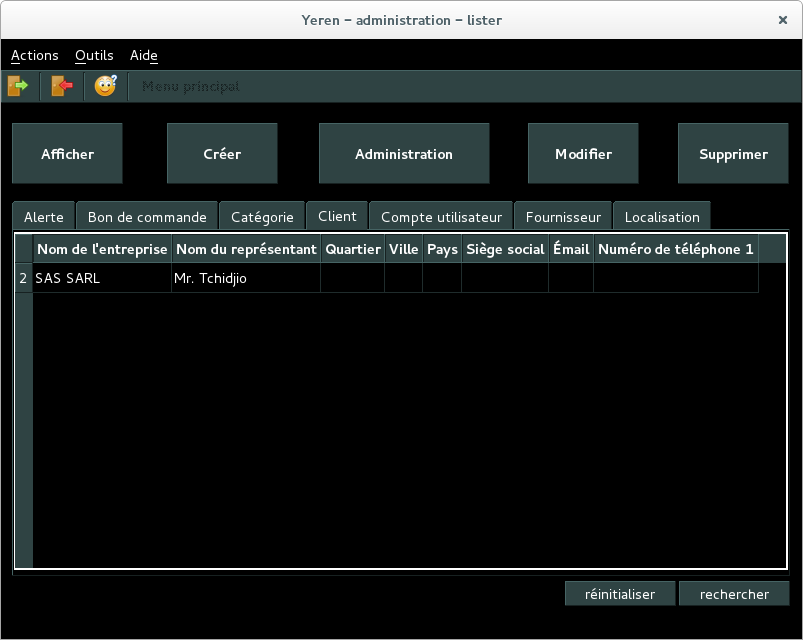
\includegraphics[scale=0.45]{images/compte-client-lister.png}
	\caption{L'interface graphique qui liste les comptes clients.}
	\label{fig:admin-comptes-clients-lister}
\end{figure}

La figure~\ref{fig:admin-comptes-clients-lister} illustre
l'interface graphique de \yeren qui liste les comptes clients.

\procparagraph{Proc\'edure pour lister les comptes clients}
\begin{enumerate}[1)]
	\item \`A partir de l'interface graphique de l'acceuil de
		l'administration (voir figure~\ref{fig:fenetre-administrateur}),
		on clique sur l'onglet intitul\'e \textbf{op\'erations}. 
		
	\item Choisir '\textbf{lister}' dans le '\emph{combo box
		op\'erations}'.
		
	\item Choisir '\textbf{un compte client}' dans
		le '\emph{combo box objets}'. Vous \^etes automatiquement
		conduit \`a la fen\^etre qui liste les comptes clients
		(figure~\ref{fig:admin-comptes-clients-lister}).
\end{enumerate}

%------------------------------------------------------------------------------

\newpage
\nxsubsection{Modifier les d\'etails d'un compte client}
\index{modifier les d\'etails d'un compte client}

\begin{figure}[!htpb]
	\centering
	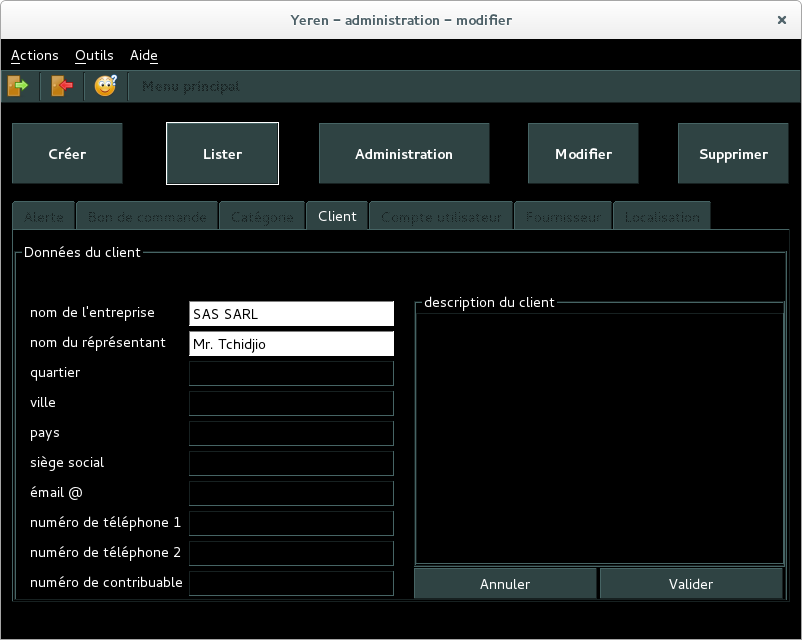
\includegraphics[scale=0.45]{images/compte-client-modifier.png}
	\caption{L'interface graphique pour modifier les d\'etails
			d'un compte client.}
	\label{fig:admin-comptes-clients-modifier}
\end{figure}

La figure~\ref{fig:admin-comptes-clients-modifier} illustre
l'interface graphique de \yeren pour modifier les
d\'etails d'un compte client.

\procparagraph{Proc\'edure pour modifier les d\'etails d'un compte client}
\begin{enumerate}[1)]
	\item \`A partir de l'interface graphique de l'acceuil de
		l'administration (voir figure~\ref{fig:fenetre-administrateur}),
		on clique sur l'onglet intitul\'e \textbf{op\'erations}. 
		
	\item Choisir '\textbf{lister}' dans le '\emph{combo box
		op\'erations}'.
		
	\item Choisir '\textbf{un compte client}' dans le '\emph{combo box
		sujets}'. Vous \^etes automatiquement conduit \`a la fen\^etre
		illustr\'ee par la figure~\ref{fig:admin-comptes-clients-lister}.
		
	\item S\'electionner le compte client dont vous souhaitez
		modifier les d\'etails dans la liste des comptes
		clients affich\'ee.
		
	\item Cliquer sur le bouton \bouton{Modifier}. Les d\'etails
		du compte client sont affich\'es dans une nouvelle fen\^etre.
		
	\item Faites les modifications que vous souhaitez.
		
	\item Cliquer sur le bouton \bouton{valider} pour valider
		les modifications faites.
\end{enumerate}

%------------------------------------------------------------------------------

\newpage
\nxsubsection{Supprimer un compte client}
\index{supprimer un compte client}

\begin{figure}[!htpb]
	\centering
	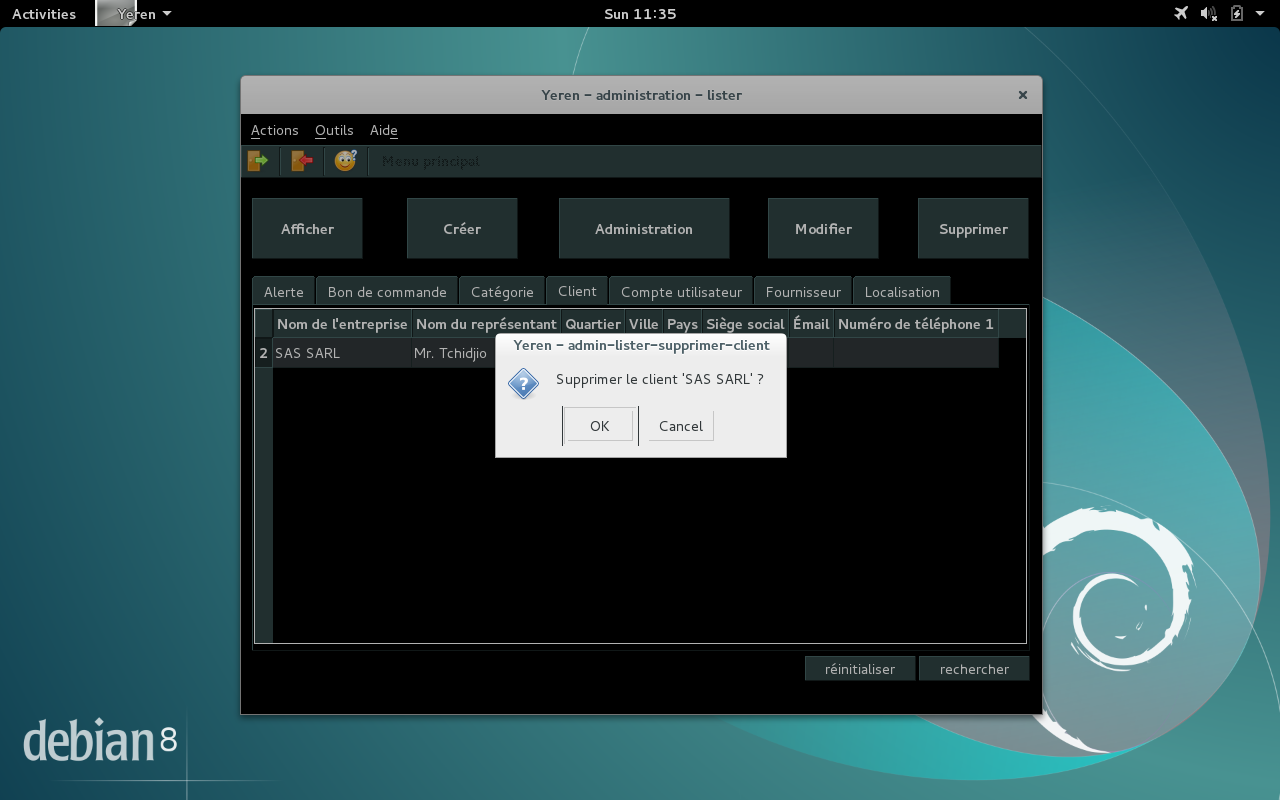
\includegraphics[scale=0.39]{images/compte-client-supprimer.png}
	\caption{L'interface graphique pour supprimer un compte client.}
	\label{fig:admin-comptes-clients-supprimer}
\end{figure}

La figure~\ref{fig:admin-comptes-clients-supprimer} illustre
l'interface graphique de \yeren pour supprimer un compte
client.

\procparagraph{Proc\'edure pour supprimer un compte client}
\begin{enumerate}[1)]
	\item \`A partir de l'interface graphique de l'acceuil de
		l'administration (voir figure~\ref{fig:fenetre-administrateur}),
		on clique sur l'onglet intitul\'e \textbf{op\'erations}. 
		
	\item Choisir '\textbf{supprimer}' dans le '\emph{combo box
		op\'erations}'.
		
	\item Choisir '\textbf{un compte client}' dans le '\emph{combo box
		sujets}'. Vous \^etes automatiquement conduit \`a la fen\^etre
		illustr\'ee par la figure~\ref{fig:admin-comptes-clients-lister}.
		
	\item S\'electionner le compte client \`a supprimer dans la liste
		des comptes clients affich\'ee.
		
	\item Cliquer sur le bouton \bouton{Supprimer}. La question
		est ensuite pos\'ee si vous confirmer votre choix.
		Cliquer sur le \bouton{OK} pour confirmer votre choix.
\end{enumerate}

\newpage

%-----------------------------------------------------------

\nxsection{Les Comptes Fournisseurs}
\index{les comptes fournisseurs}

\nxsubsection{Afficher les d\'etails d'un compte fournisseur}
\index{afficher les d\'etails d'un compte fournisseur}
\index{d\'etails d'un compte fournisseur}

\begin{figure}[!htpb]
	\centering
	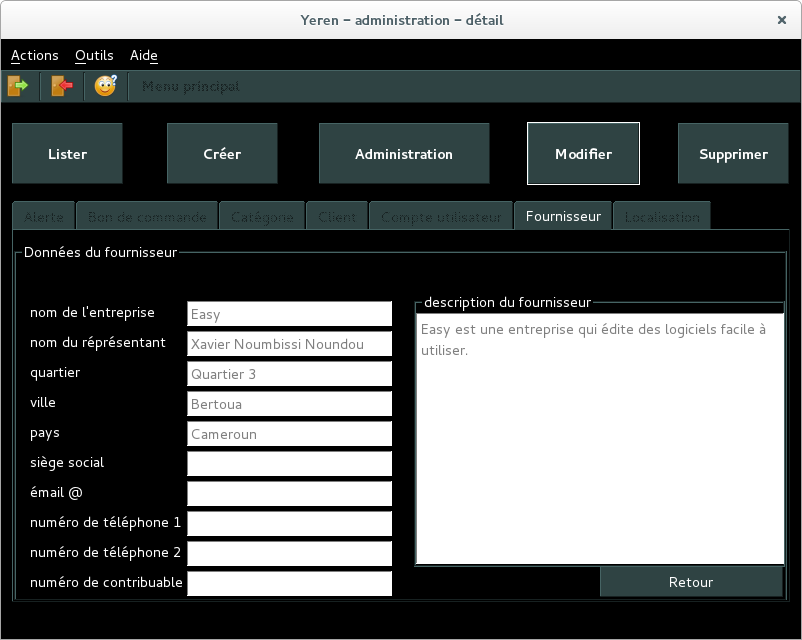
\includegraphics[scale=0.45]{images/compte-fournisseur-afficher-details.png}
	\caption{L'interface graphique pour afficher les d\'etails
			d'un compte fournisseur.}
	\label{fig:admin-fournisseurs-afficher-details}
\end{figure}

La figure~\ref{fig:admin-fournisseurs-afficher-details}
illustre l'interface graphique de \yeroth qui affiche
les d\'etails d'un compte fournisseur.

\procparagraph{Proc\'edure pour afficher les d\'etails
	d'un compte fournisseur}
\begin{enumerate}[1)]
	\item \`A partir de l'interface graphique de l'acceuil de
		l'administration (voir figure~\ref{fig:fenetre-administrateur}),
		on clique sur l'onglet intitul\'e \textbf{op\'erations}. 
		
	\item Choisir '\textbf{lister}' dans le '\emph{combo box
		op\'erations}'.
		
	\item Choisir '\textbf{un compte fournisseur}' dans le
		'\emph{combo box objets}'. Vous \^etes automatiquement
		conduit \`a la fen\^etre illustr\'ee par la
		figure~\ref{fig:admin-comptes-fournisseurs-lister}.
		
	\item S\'electionner le compte fournisseur dont vous
		souhaitez afficher les d\'etails dans la liste des
		comptes fournisseurs affich\'ee.
		
	\item Cliquer sur le bouton \bouton{Afficher}. Les d\'etails
		sur le compte fournisseur sont affich\'es dans une nouvelle.
\end{enumerate}

%%%%%%%%%%%%%%%%%%%%%%%%%%%%%%%%%%%%%%%%%%%%%%%%%%%%%%%%%%%%%%%%%%%%%%%%%%%%%%%%%

\newpage
\nxsubsection{Cr\'eer un compte fournisseur}
\index{cr\'eer un compte fournisseur}

\begin{figure}[!htpb]
	\centering
	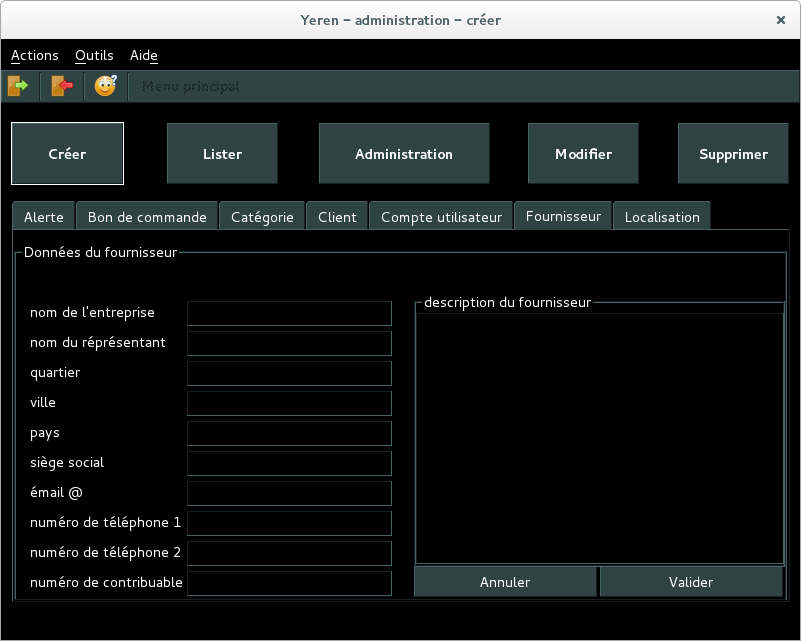
\includegraphics[scale=0.45]{images/compte-fournisseur-creer.png}
	\caption{L'interface graphique pour cr\'eer un
			nouveau compte fournisseur.}
	\label{fig:admin-comptes-fournisseurs-creer}
\end{figure}

La figure~\ref{fig:admin-comptes-fournisseurs-creer} illustre
l'interface graphique de \yeroth pour cr\'eer un nouveau
compte fournisseur.

\procparagraph{Proc\'edure pour cr\'eer un compte fournisseur}
\begin{enumerate}[1)]
	\item \`A partir de l'interface graphique de l'acceuil de
		l'administration (voir figure~\ref{fig:fenetre-administrateur}),
		on clique sur l'onglet intitul\'e \textbf{op\'erations}. 
		
	\item Choisir '\textbf{cr\'eer}' dans le '\emph{combo box
		op\'erations}'.
		
	\item Choisir '\textbf{un compte fournisseur}' dans
		le '\emph{combo box objets}'. Vous \^etes automatiquement
		conduit \`a la fen\^etre illustr\'ee par la
		figure~\ref{fig:admin-comptes-fournisseurs-creer}.
		
	\item Saisissez les informations requises dans les champs de texte
		suivants:
		\begin{enumerate}[1)]
			\item nom de l'entreprise \obligatoire
			\item nom du r\'epr\'esentant
			\item quartier
			\item ville 
			\item pays
			\item si\`ege social
			\item \'email@
			\item num\'ero de t\'el\'ephone 1
			\item num\'ero de t\'el\'ephone 2
			\item num\'ero de contribuable 
			\item description du fournisseur.
		\end{enumerate}
		
	\item Cliquer sur le bouton \bouton{Valider} pour
		valider votre travail.		
\end{enumerate}

%%%%%%%%%%%%%%%%%%%%%%%%%%%%%%%%%%%%%%%%%%%%%%%%%%%%%%%%%%%%%%%%%%%%%%%%%%%%%%%%%

\newpage
\nxsubsection{Lister les fournisseurs}
\index{lister les fournisseurs}

\begin{figure}[!htpb]
	\centering
	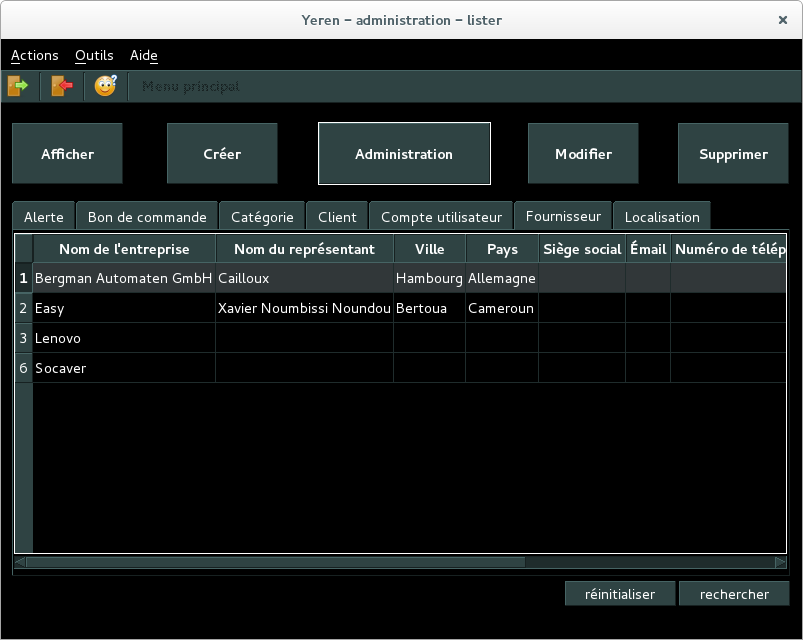
\includegraphics[scale=0.45]{images/compte-fournisseur-lister.png}
	\caption{L'interface graphique pour lister les comptes fournisseurs.}
	\label{fig:admin-comptes-fournisseurs-lister}
\end{figure}

La figure~\ref{fig:admin-comptes-fournisseurs-lister} illustre
l'interface graphique de \yeroth qui liste les comptes fournisseurs.

\procparagraph{Proc\'edure pour lister les comptes fournisseurs}
\begin{enumerate}[1)]
	\item \`A partir de l'interface graphique de l'acceuil de
		l'administration (voir figure~\ref{fig:fenetre-administrateur}),
		on clique sur l'onglet intitul\'e \textbf{op\'erations}. 
		
	\item Choisir '\textbf{lister}' dans le '\emph{combo box
		op\'erations}'.
		
	\item Choisir '\textbf{un compte fournisseur}' dans
		le '\emph{combo box objets}'. Vous \^etes automatiquement
		conduit \`a la fen\^etre qui liste les comptes fournisseurs
		(figure~\ref{fig:admin-comptes-fournisseurs-lister}).
\end{enumerate}

%%%%%%%%%%%%%%%%%%%%%%%%%%%%%%%%%%%%%%%%%%%%%%%%%%%%%%%%%%%%%%%%%%%%%%%%%%%%%%%%%

\newpage
\nxsubsection{Modifier les d\'etails d'un fournisseur}
\index{modifier les d\'etails d'un fournisseur}

\begin{figure}[!htpb]
	\centering
	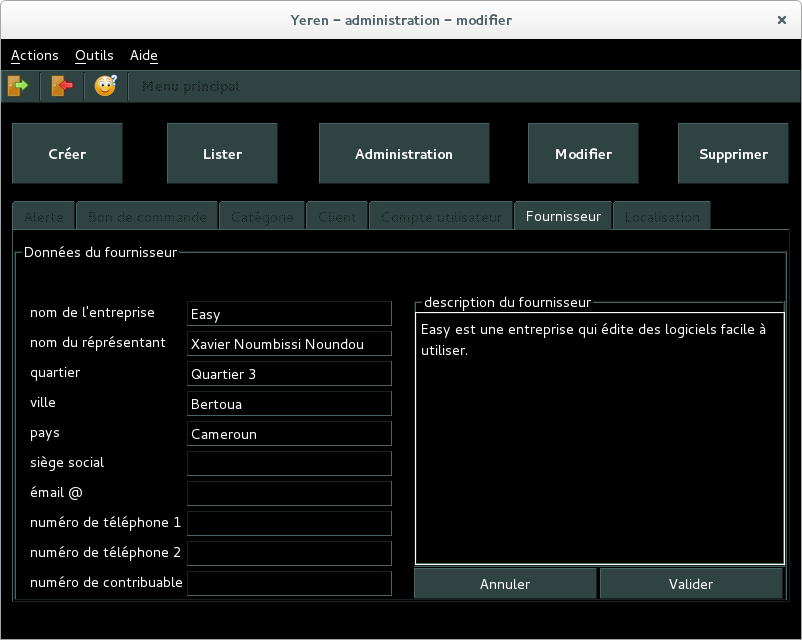
\includegraphics[scale=0.45]{images/compte-fournisseur-modifier.png}
	\caption{L'interface graphique pour modifier les
			d\'etails d'un compte fournisseur.}
	\label{fig:admin-comptes-fournisseurs-modifier}
\end{figure}

La figure~\ref{fig:admin-comptes-fournisseurs-modifier} illustre
l'interface graphique de \yeroth pour modifier les
d\'etails d'un compte fournisseur.

\procparagraph{Proc\'edure pour modifier les d\'etails d'un compte fournisseur}
\begin{enumerate}[1)]
	\item \`A partir de l'interface graphique de l'acceuil de
		l'administration (voir figure~\ref{fig:fenetre-administrateur}),
		on clique sur l'onglet intitul\'e \textbf{op\'erations}. 
		
	\item Choisir '\textbf{lister}' dans le '\emph{combo box
		op\'erations}'.
		
	\item Choisir '\textbf{un compte fournisseur}' dans le '\emph{combo box
		sujets}'. Vous \^etes automatiquement conduit \`a la fen\^etre
		illustr\'ee par la figure~\ref{fig:admin-comptes-fournisseurs-lister}.
		
	\item S\'electionner le compte fournisseur dont vous souhaitez
		modifier les d\'etails dans la liste des comptes fournisseurs
		affich\'ee.
		
	\item Cliquer sur le bouton \bouton{Modifier}. Les d\'etails
		du compte fournisseur sont affich\'es dans une nouvelle fen\^etre.
		
	\item Faites les modifications que vous souhaitez.
		
	\item Cliquer sur le bouton \bouton{valider} pour valider
		les modifications faites.
\end{enumerate}

%%%%%%%%%%%%%%%%%%%%%%%%%%%%%%%%%%%%%%%%%%%%%%%%%%%%%%%%%%%%%%%%%%%%%%%%%%%%%%%%%

\newpage
\nxsubsection{Supprimer un compte fournisseur}
\index{supprimer un compte fournisseur}

\begin{figure}[!htpb]
	\centering
	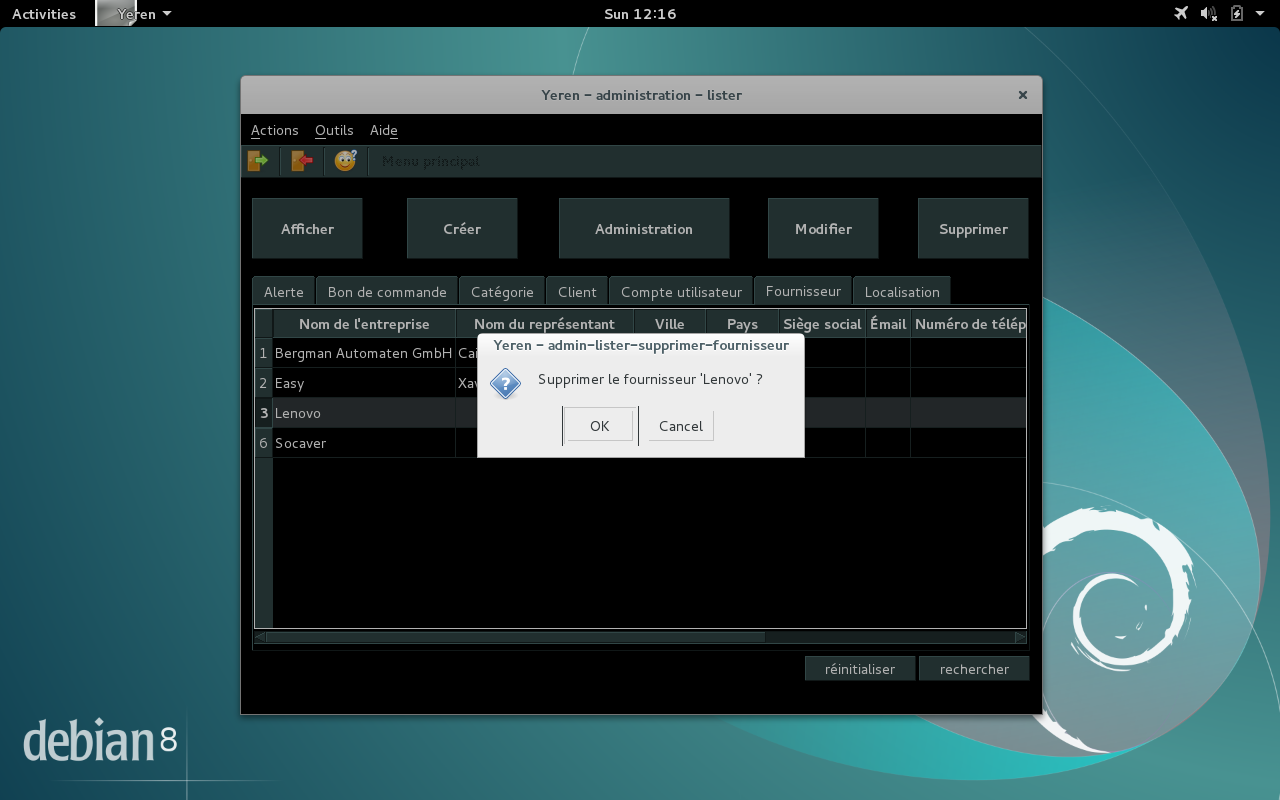
\includegraphics[scale=0.39]{images/compte-fournisseur-supprimer.png}
	\caption{L'interface graphique pour supprimer un fournisseur.}
	\label{fig:admin-comptes-fournisseurs-supprimer}
\end{figure}

La figure~\ref{fig:admin-comptes-fournisseurs-supprimer}
illustre l'interface graphique de \yeroth pour supprimer
un compte fournisseur.

\procparagraph{Proc\'edure pour supprimer un compte fournisseur}
\begin{enumerate}[1)]
	\item \`A partir de l'interface graphique de l'acceuil de
		l'administration (voir figure~\ref{fig:fenetre-administrateur}),
		on clique sur l'onglet intitul\'e \textbf{op\'erations}. 
		
	\item Choisir '\textbf{supprimer}' dans le '\emph{combo box
		op\'erations}'.
		
	\item Choisir '\textbf{un compte fournisseur}' dans le
		'\emph{combo box objets}'. Vous \^etes automatiquement
		conduit \`a la fen\^etre illustr\'ee par la
		figure~\ref{fig:admin-comptes-fournisseurs-lister}.
		
	\item S\'electionner le compte fournisseur \`a supprimer
		dans la liste des comptes fournisseurs affich\'ee.
		
	\item Cliquer sur le bouton \bouton{Supprimer}. La question
		est ensuite pos\'ee si vous confirmer votre choix.
		Cliquer sur le \bouton{OK} pour confirmer votre choix.
\end{enumerate}

\newpage

%-----------------------------------------------------------

\nxsection{Les Comptes Utilisateurs}
\index{les comptes utilisateurs}

\nxsubsection{Afficher les d\'etails d'un compte utilisateur}
\index{afficher les d\'etails d'un compte utilisateur}
\index{d\'etails d'un compte utilisateur}

\begin{figure}[!htpb]
	\centering
	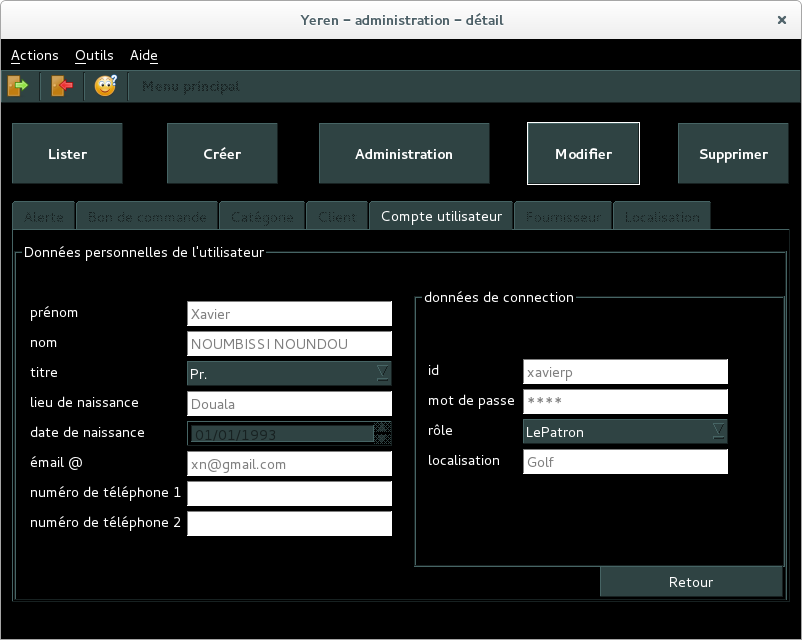
\includegraphics[scale=0.45]{images/compte-utilisateur-afficher-details.png}
	\caption{L'interface graphique pour afficher les d\'etails
			d'un compte utilisateur.}
	\label{fig:admin-comptes-utilisateurs-afficher-details}
\end{figure}

La figure~\ref{fig:admin-comptes-utilisateurs-afficher-details}
illustre l'interface graphique de \yeroth qui affiche les
d\'etails d'un compte utilisateur.

\procparagraph{Proc\'edure pour afficher les d\'etails d'un compte utilisateur}
\begin{enumerate}[1)]
	\item \`A partir de l'interface graphique de l'acceuil de
		l'administration (voir figure~\ref{fig:fenetre-administrateur}),
		on clique sur l'onglet intitul\'e \textbf{op\'erations}. 
		
	\item Choisir '\textbf{lister}' dans le '\emph{combo box
		op\'erations}'.
		
	\item Choisir '\textbf{un compte utilisateur}' dans le
		'\emph{combo box objets}'. Vous \^etes automatiquement
		conduit \`a la fen\^etre illustr\'ee par la
		figure~\ref{fig:admin-comptes-utilisateurs-lister}.
		
	\item S\'electionner le compte utilisateur dont vous
		souhaitez afficher les d\'etails dans la liste des
		comptes utilisateurs affich\'ee.
		
	\item Cliquer sur le bouton \bouton{Afficher}. Les d\'etails
		sur le compte utilisateur sont affich\'es dans
		une nouvelle fen\^etre.
\end{enumerate}

%%%%%%%%%%%%%%%%%%%%%%%%%%%%%%%%%%%%%%%%%%%%%%%%%%%%%%%%%%%%%%%%%%%%%%%%%%%%%%%%%

\newpage
\nxsubsection{Cr\'eer un compte utilisateur}
\index{cr\'eer un compte utilisateur}

\begin{figure}[!htpb]
	\centering
	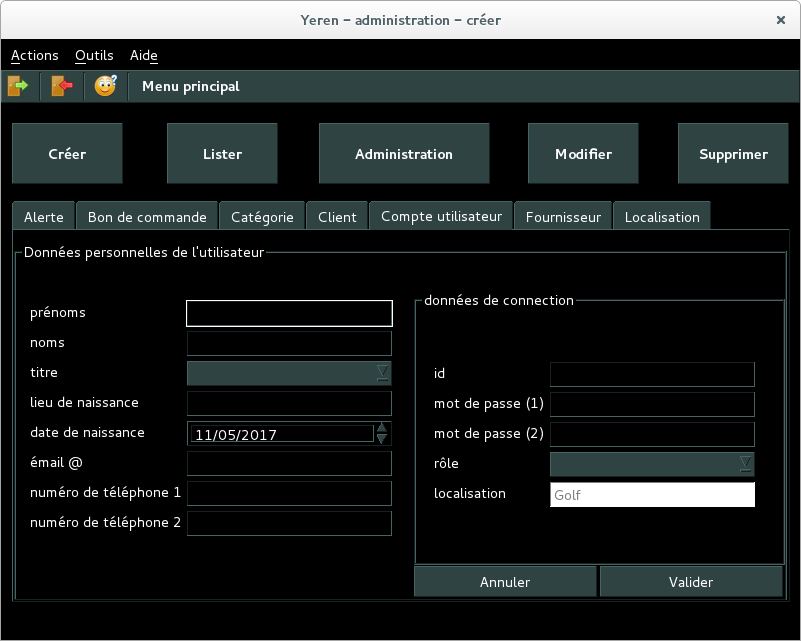
\includegraphics[scale=0.45]{images/compte-utilisateur-creer.png}
	\caption{L'interface graphique pour cr\'eer un compte utilisateur.}
	\label{fig:admin-comptes-utilisateurs-creer}
\end{figure}

La figure~\ref{fig:admin-comptes-utilisateurs-creer} illustre
l'interface graphique de \yeroth pour cr\'eer un nouveau
compte utilisateur.

\procparagraph{Proc\'edure pour cr\'eer un compte utilisateur}
\begin{enumerate}[1)]
	\item \`A partir de l'interface graphique de l'acceuil de
		l'administration (voir figure~\ref{fig:fenetre-administrateur}),
		on clique sur l'onglet intitul\'e \textbf{op\'erations}. 
		
	\item Choisir '\textbf{cr\'eer}' dans le '\emph{combo box
		op\'erations}'.
		
	\item Choisir '\textbf{un compte utilisateur}' dans
		le '\emph{combo box objets}'. Vous \^etes automatiquement
		conduit \`a la fen\^etre illustr\'ee par la
		figure~\ref{fig:admin-comptes-utilisateurs-creer}.
		
	\item Saisissez les informations requises dans les champs
		de texte suivants:
		\begin{enumerate}[1)]
			\item pr\'enoms \obligatoire
			\item noms \obligatoire
			\item titre	\obligatoire
			\item lieu de naissance 
			\item date de naissance
			\item ville
			\item province / \'etat
			\item pays
			\item bo\^ite postale
			\item \'email 
			\item num\'ero de t\'el\'ephone 1 
			\item num\'ero de t\'el\'ephone 2 
			\item nom d'utilisateur \obligatoire
			\item mot de passe \obligatoire
			\item v\'erification du mot de passe \obligatoire			
			\item r\^ole \obligatoire.
		\end{enumerate}
		
	\item Cliquer sur le bouton \bouton{Valider} pour
		valider votre travail.	
\end{enumerate}


%%%%%%%%%%%%%%%%%%%%%%%%%%%%%%%%%%%%%%%%%%%%%%%%%%%%%%%%%%%%%%%%%%%%%%%%%%%%%%%%%

\newpage
\nxsubsection{Lister les comptes utilisateurs}
\index{lister les comptes utilisateur}

\begin{figure}[!htpb]
	\centering
	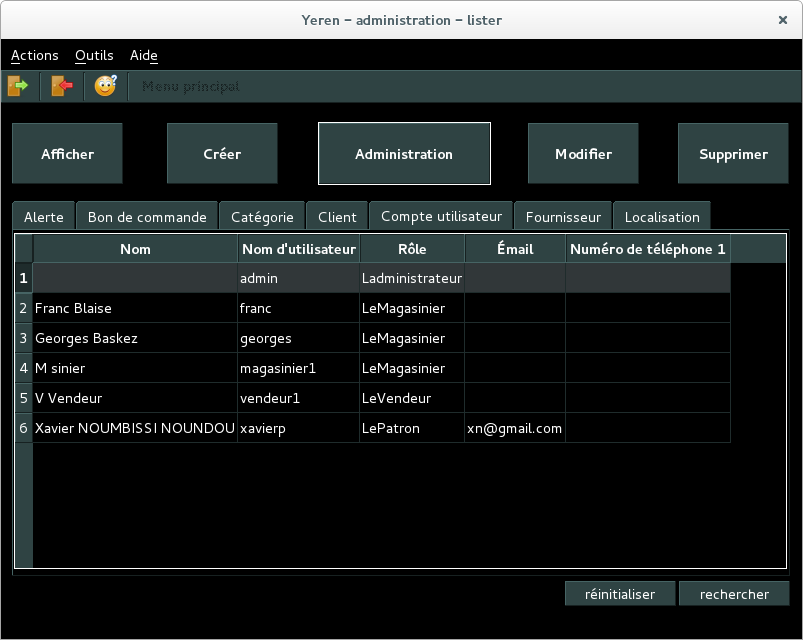
\includegraphics[scale=0.45]{images/compte-utilisateur-lister.png}
	\caption{L'interface graphique pour lister les comptes utilisateurs.}
	\label{fig:admin-comptes-utilisateurs-lister}
\end{figure}

La figure~\ref{fig:admin-comptes-utilisateurs-lister}
illustre l'interface graphique de \yeroth qui liste les
comptes utilisateurs.

\procparagraph{Proc\'edure pour lister les comptes utilisateurs}
\begin{enumerate}[1)]
	\item \`A partir de l'interface graphique de l'acceuil de
		l'administration (voir figure~\ref{fig:fenetre-administrateur}),
		on clique sur l'onglet intitul\'e \textbf{op\'erations}. 
		
	\item Choisir '\textbf{lister}' dans le '\emph{combo box
		op\'erations}'.
		
	\item Choisir '\textbf{un compte utilisateur}' dans
		le '\emph{combo box objets}'. Vous \^etes automatiquement
		conduit \`a la fen\^etre qui liste les comptes clients
		(figure~\ref{fig:admin-comptes-utilisateurs-lister}).
\end{enumerate}

%%%%%%%%%%%%%%%%%%%%%%%%%%%%%%%%%%%%%%%%%%%%%%%%%%%%%%%%%%%%%%%%%%%%%%%%%%%%%%%%%

\newpage
\nxsubsection{Modifier les d\'etails d'un compte utilisateur}
\index{modifier les d\'etails d'un compte utilisateur}

\begin{figure}[!htpb]
	\centering
	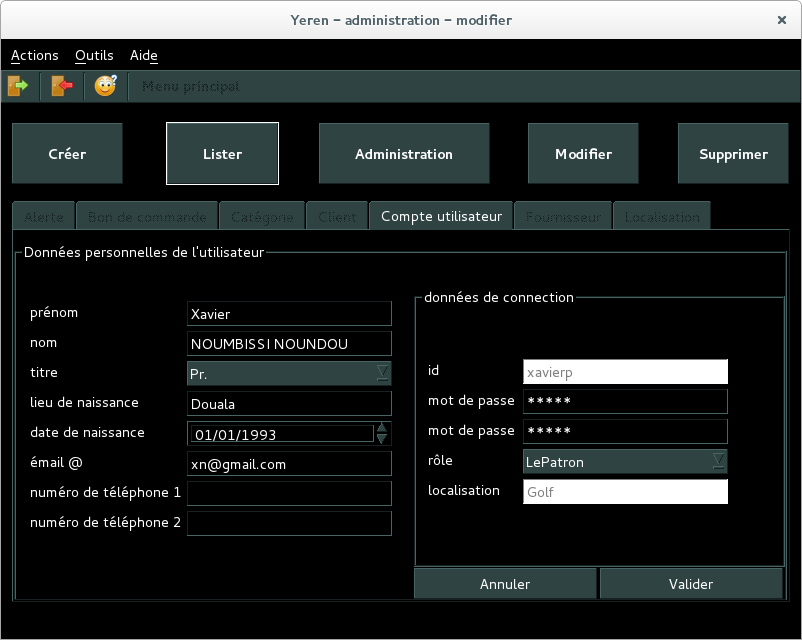
\includegraphics[scale=0.45]{images/compte-utilisateur-modifier.png}
	\caption{L'interface graphique pour modifier les d\'etails
			d'un compte utilisateur.}
	\label{fig:admin-comptes-utilisateurs-modifier}
\end{figure}

La figure~\ref{fig:admin-comptes-utilisateurs-modifier} illustre
l'interface graphique de \yeroth pour modifier les d\'etails
d'un compte utilisateur.

\procparagraph{Proc\'edure pour modifier les d\'etails d'un compte utilisateur}
\begin{enumerate}[1)]
	\item \`A partir de l'interface graphique de l'acceuil de
		l'administration (voir figure~\ref{fig:fenetre-administrateur}),
		on clique sur l'onglet intitul\'e \textbf{op\'erations}. 
		
	\item Choisir '\textbf{lister}' dans le '\emph{combo box
		op\'erations}'.
		
	\item Choisir '\textbf{un compte utilisateur}' dans
		le '\emph{combo box objets}'. Vous \^etes automatiquement
		conduit \`a la fen\^etre illustr\'ee par la
		figure~\ref{fig:admin-comptes-utilisateurs-lister}.
		
	\item S\'electionner le compte utilisateur dont vous souhaitez
		modifier les d\'etails dans la liste des comptes
		utilisateurs affich\'ee.
		
	\item Cliquer sur le bouton \bouton{Modifier}. Les d\'etails
		du compte utilisateur sont affich\'es dans une nouvelle fen\^etre.
		
	\item Faites les modifications que vous souhaitez.
		
	\item Cliquer sur le bouton \bouton{valider} pour valider
		les modifications faites.
\end{enumerate}

%%%%%%%%%%%%%%%%%%%%%%%%%%%%%%%%%%%%%%%%%%%%%%%%%%%%%%%%%%%%%%%%%%%%%%%%%%%%%%%%%

\newpage
\nxsubsection{Supprimer un compte utilisateur}
\index{supprimer un compte utilisateur}

\begin{figure}[!htpb]
	\centering
	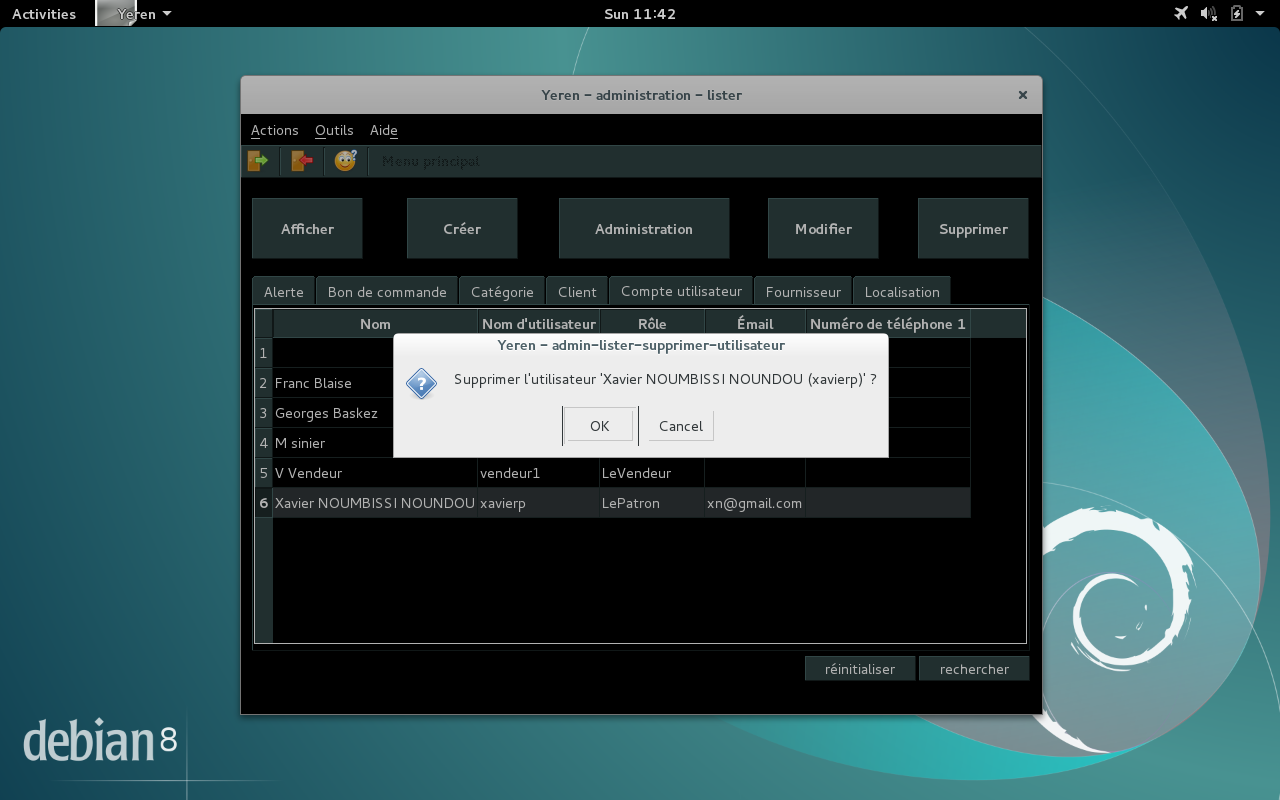
\includegraphics[scale=0.39]{images/compte-utilisateur-supprimer.png}
	\caption{L'interface graphique pour supprimer un compte utilisateur.}
	\label{fig:admin-comptes-utilisateurs-supprimer}
\end{figure}

La figure~\ref{fig:admin-comptes-utilisateurs-supprimer}
illustre l'interface graphique de \yeroth pour supprimer
un compte utilisateur.

\procparagraph{Proc\'edure pour supprimer un compte utilisateur}
\begin{enumerate}[1)]
	\item \`A partir de l'interface graphique de l'acceuil de
		l'administration (voir figure~\ref{fig:fenetre-administrateur}),
		on clique sur l'onglet intitul\'e \textbf{op\'erations}. 
		
	\item Choisir '\textbf{supprimer}' dans le '\emph{combo box
		op\'erations}'.
		
	\item Choisir '\textbf{un compte utilisateur}' dans le
		'\emph{combo box objets}'. Vous \^etes automatiquement
		conduit \`a la fen\^etre illustr\'ee par la
		figure~\ref{fig:admin-comptes-utilisateurs-lister}.
		
	\item S\'electionner le compte utilisateur \`a supprimer
		dans la liste des comptes utilisateurs affich\'ee.
		
	\item Cliquer sur le bouton \bouton{Supprimer}. La question
		est ensuite pos\'ee si vous confirmer votre choix.
		Cliquer sur le \bouton{OK} pour confirmer votre choix.
\end{enumerate}

\newpage

%-----------------------------------------------------------

\nxsection{Les Localisations}
\index{localisation}

Une localisation repr\'esente une boutique ou un d\'ep\^ot
de l'entreprise utilisant \yeren.

Les informations sur une localisation permettent de
se connecter \`a la base de donn\'ees de la boutique
ou du d\'ep\^ot qu'elle repr\'esente.

\nxsubsection{Afficher les d\'etails d'une localisation}
\index{afficher les d\'etails d'une localisation}
\index{d\'etails d'une localisation}

La figure~\ref{fig:admin-localisations-afficher-details} illustre
l'interface graphique de \yeren qui affiche les d\'etails
d'une localisation.\\

\begin{figure}[!htpb]
	\centering
	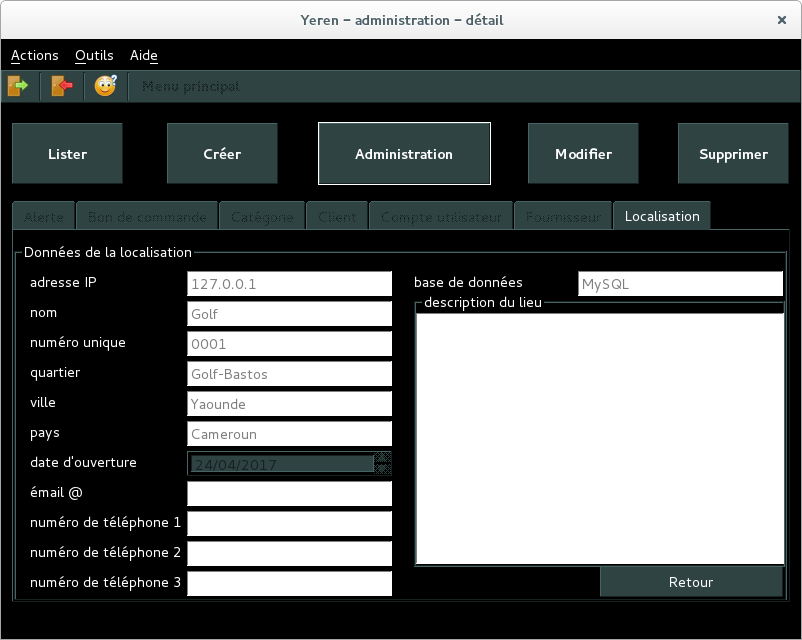
\includegraphics[scale=0.45]{images/localisation-afficher-details.png}
	\caption{L'interface graphique pour afficher les d\'etails
			d'une localisation.}
	\label{fig:admin-localisations-afficher-details}
\end{figure}

\procparagraph{Proc\'edure pour afficher les d\'etails d'une localisation}
\begin{enumerate}[1)]
	\item \`A partir de l'interface graphique de l'acceuil de
		l'administration (voir figure~\ref{fig:fenetre-administrateur}),
		on clique sur l'onglet intitul\'e \textbf{op\'erations}. 
		
	\item Choisir '\textbf{lister}' dans le '\emph{combo box
		op\'erations}'.
		
	\item Choisir '\textbf{une localisation}' dans le '\emph{combo box
		sujets}'. Vous \^etes automatiquement conduit \`a la fen\^etre
		illustr\'ee par la figure~\ref{fig:admin-localisations-lister}.
		
	\item S\'electionner la localisation dont vous souhaitez afficher
		les d\'etails dans la liste des localisations affich\'ee.
		
	\item Cliquer sur le bouton \bouton{Afficher}. Les d\'etails
		sur la localisation choisie sont affich\'es dans
		une nouvelle fen\^etre.
\end{enumerate}

%%%%%%%%%%%%%%%%%%%%%%%%%%%%%%%%%%%%%%%%%%%%%%%%%%%%%%%%%%%%%%%%%%%%%%%%%%%%%%%%%

\nxsubsection{Cr\'eer une localisation}
\index{cr\'eer une localisation}

La figure~\ref{fig:admin-localisations-creer} illustre
l'interface graphique de \yeren pour cr\'eer une localisation.\\

\begin{figure}[!htpb]
	\centering
	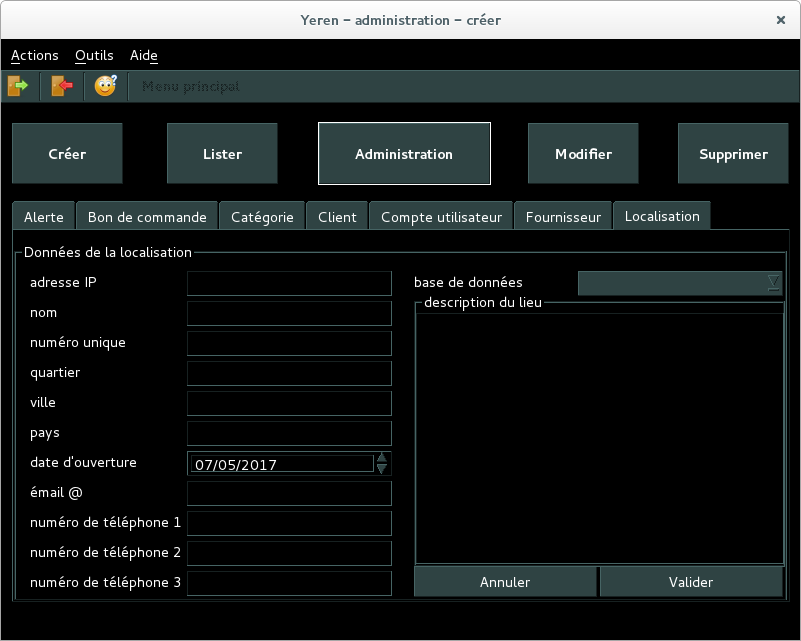
\includegraphics[scale=0.45]{images/localisation-creer.png}
	\caption{L'interface graphique pour cr\'eer une localisation.}
	\label{fig:admin-localisations-creer}
\end{figure}

\procparagraph{Proc\'edure pour cr\'eer une localisation}
\begin{enumerate}[1)]
	\item \`A partir de l'interface graphique de l'acceuil de
		l'administration (voir figure~\ref{fig:fenetre-administrateur}),
		on clique sur l'onglet intitul\'e \textbf{op\'erations}. 
		
	\item Choisir '\textbf{cr\'eer}' dans le '\emph{combo box
		op\'erations}'.
		
	\item Choisir '\textbf{une localisation}' dans
		le '\emph{combo box objets}'. Vous \^etes automatiquement
		conduit \`a la fen\^etre illustr\'ee par la
		figure~\ref{fig:admin-localisations-creer}.
		
	\item Saisissez les informations requises dans les champs
		de texte suivants:
		\begin{enumerate}[1)]
			\item adresse IP 
			\item nom \obligatoire
			\item num\'ero unique 
			\item quartier
			\item ville
			\item province / \'etat
			\item pays
			\item bo\^ite postale
			\item date d'ouverture
			\item \'email@
			\item num\'ero de t\'el\'ephone 1
			\item num\'ero de t\'el\'ephone 2	
			\item base de donn\'ees					
			\item description du lieu.\\
		\end{enumerate}
		
		Si vous avez entr\'e une adresse IP pour cette 
		localisation, vous devez choisir le type de base de
		donn\'ees utilis\'e dans cette localisation. Pour
		l'instant, \yeren ne fonctionne qu'avec \emphbf{MySQL}.\\
		
		La section~\ref{sec:yeren-sgbd} dans
		l'annexe~\ref{chap:environement-logiciel-requis}
		(L'Environnement Logiciel) contient plus d'information
		aux sujets des bases de donn\'ees dans \yeren.
		
	\item Cliquer sur le bouton \bouton{Valider} pour
		valider votre travail.	
\end{enumerate}

%%%%%%%%%%%%%%%%%%%%%%%%%%%%%%%%%%%%%%%%%%%%%%%%%%%%%%%%%%%%%%%%%%%%%%%%%%%%%%%%%

\newpage
\nxsubsection{Lister les localisations}
\index{lister les localisations}

La figure~\ref{fig:admin-localisations-lister} illustre
l'interface graphique de \yeren qui liste les localisations.\\

\begin{figure}[!htpb]
	\centering
	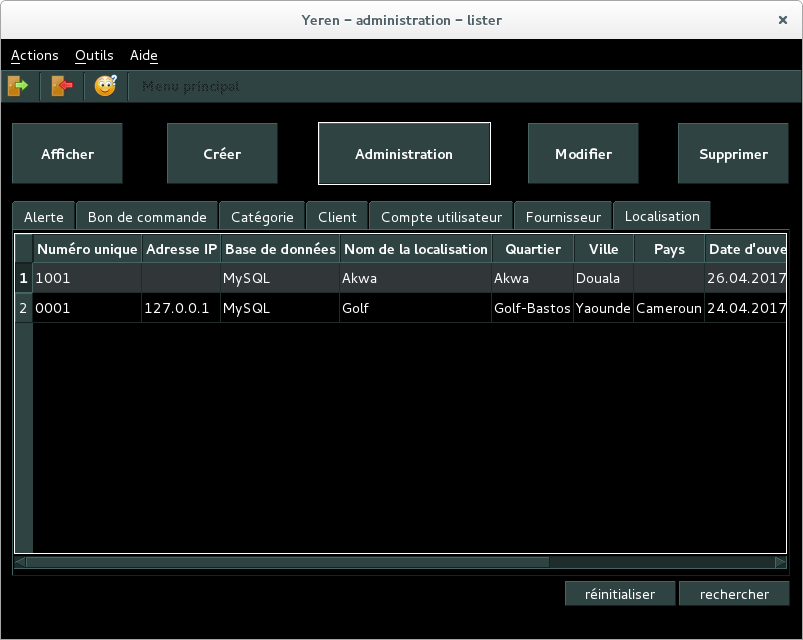
\includegraphics[scale=0.45]{images/localisation-lister.png}
	\caption{L'interface graphique pour cr\'eer une localisation.}
	\label{fig:admin-localisations-lister}
\end{figure}

\procparagraph{Proc\'edure pour lister les localisations}
\begin{enumerate}[1)]
	\item \`A partir de l'interface graphique de l'acceuil de
		l'administration (voir figure~\ref{fig:fenetre-administrateur}),
		on clique sur l'onglet intitul\'e \textbf{op\'erations}. 
		
	\item Choisir '\textbf{lister}' dans le '\emph{combo box
		op\'erations}'.
		
	\item Choisir '\textbf{une localisation}' dans le
		'\emph{combo box objets}'. Vous \^etes automatiquement
		conduit \`a la fen\^etre qui liste localisations
		(figure~\ref{fig:admin-localisations-lister}).
\end{enumerate}

%%%%%%%%%%%%%%%%%%%%%%%%%%%%%%%%%%%%%%%%%%%%%%%%%%%%%%%%%%%%%%%%%%%%%%%%%%%%%%%%%

\newpage
\nxsubsection{Modifier les d\'etails d'une localisation}
\index{modifier les d\'etails d'une localisation}

La figure~\ref{fig:admin-localisations-modifier} illustre
l'interface graphique de \yeren pour modifier les d\'etails
d'une localisation.\\

\begin{figure}[!htpb]
	\centering
	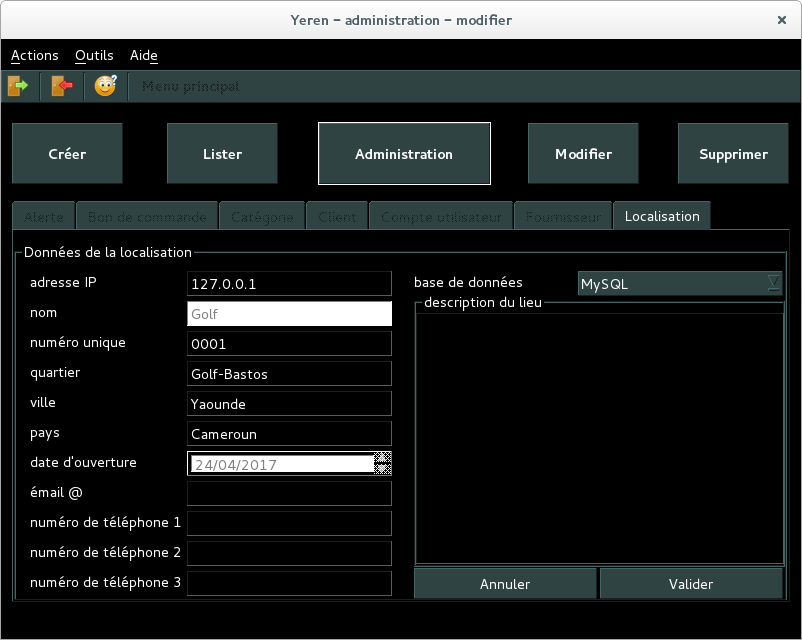
\includegraphics[scale=0.45]{images/localisation-modifier.png}
	\caption{L'interface graphique pour modifier les d\'etails
			d'une localisation.}
	\label{fig:admin-localisations-modifier}
\end{figure}

\procparagraph{Proc\'edure pour modifier les d\'etails d'une localisation}
\begin{enumerate}[1)]
	\item \`A partir de l'interface graphique de l'acceuil de
		l'administration (voir figure~\ref{fig:fenetre-administrateur}),
		on clique sur l'onglet intitul\'e \textbf{op\'erations}. 
		
	\item Choisir '\textbf{lister}' dans le '\emph{combo box
		op\'erations}'.
		
	\item Choisir '\textbf{une localisation}' dans
		le '\emph{combo box objets}'. Vous \^etes automatiquement
		conduit \`a la fen\^etre illustr\'ee par la
		figure~\ref{fig:admin-localisations-lister}.
		
	\item S\'electionner la localisation dont vous souhaitez
		modifier les d\'etails dans la liste des localisations
		affich\'ee.
		
	\item Cliquer sur le bouton \bouton{Modifier}. Les d\'etails
		de la localisation sont affich\'es dans une nouvelle
		fen\^etre.
		
	\item Faites les modifications que vous souhaitez.
		
	\item Cliquer sur le bouton \bouton{valider} pour valider
		les modifications faites.
\end{enumerate}

%%%%%%%%%%%%%%%%%%%%%%%%%%%%%%%%%%%%%%%%%%%%%%%%%%%%%%%%%%%%%%%%%%%%%%%%%%%%%%%%%

%\newpage
\nxsubsection{Supprimer une localisation}
\index{supprimer une localisation}

La figure~\ref{fig:admin-localisations-supprimer} illustre
l'interface graphique de \yeren pour supprimer une localisation.\\

\begin{figure}[!htpb]
	\centering
	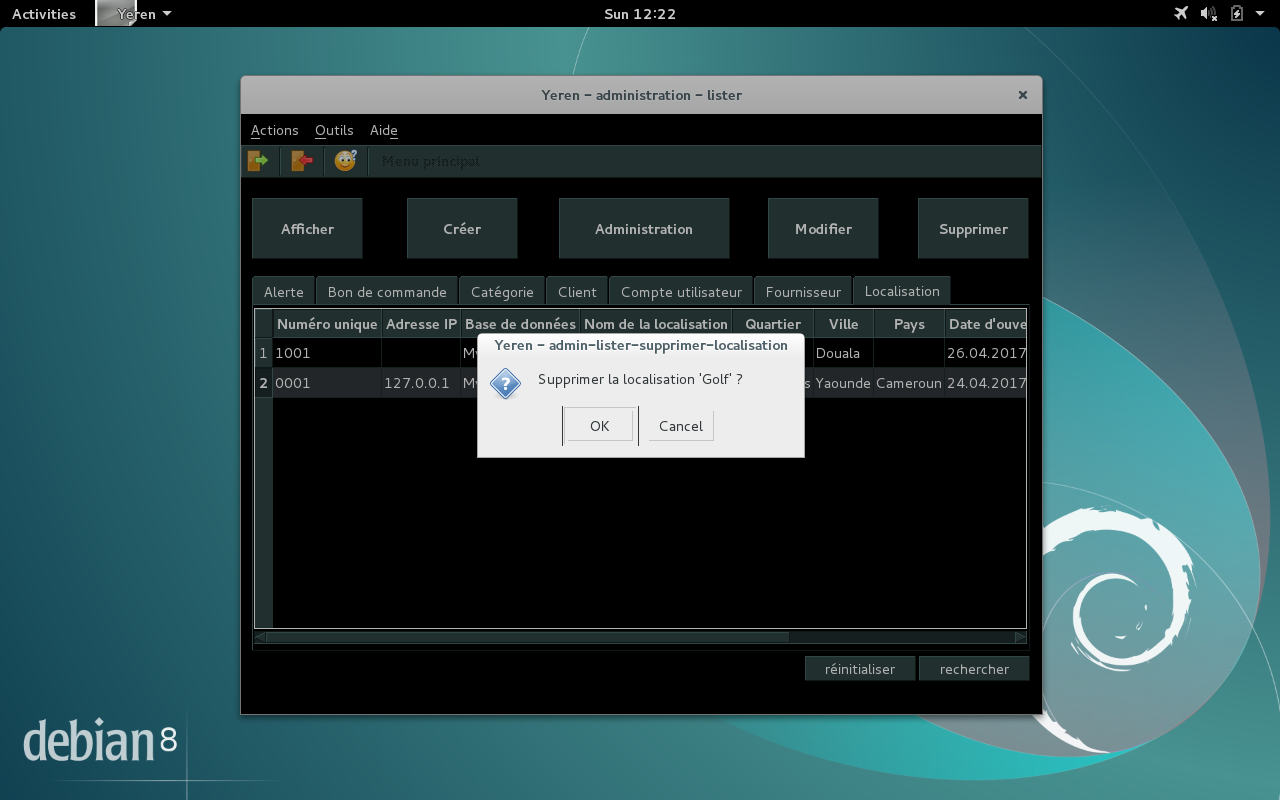
\includegraphics[scale=0.35]{images/localisation-supprimer.png}
	\caption{L'interface graphique pour supprimer une localisation.}
	\label{fig:admin-localisations-supprimer}
\end{figure}

\procparagraph{Proc\'edure pour supprimer une localisation}
\begin{enumerate}[1)]
	\item \`A partir de l'interface graphique de l'acceuil de
		l'administration (voir figure~\ref{fig:fenetre-administrateur}),
		on clique sur l'onglet intitul\'e \textbf{op\'erations}. 
		
	\item Choisir '\textbf{supprimer}' dans le '\emph{combo box
		op\'erations}'.
		
	\item Choisir '\textbf{une localisation}' dans le '\emph{combo box
		sujets}'. Vous \^etes automatiquement conduit \`a la fen\^etre
		illustr\'ee par la figure~\ref{fig:admin-localisations-lister}.
		
	\item S\'electionner la localisation \`a supprimer dans la liste
		des localisations affich\'ee.
		
	\item Cliquer sur le bouton \bouton{Supprimer}. La question
		est ensuite pos\'ee si vous confirmer votre choix.
		Cliquer sur le \bouton{OK} pour confirmer votre choix.
\end{enumerate}


%-----------------------------------------------------------

\chapter{Les Probl\`emes Connues et leurs Solutions}\label{chap:problemes-connues}
\index{probl\`emes connues ! solutions}
\index{probl\`emes connues et solutions}

\chapintro{Ce chapitre d\'ecrit quelques
probl\`emes qui peuvent survenir lors de
l'utilisation de \yeren et comment les r\'esoudre.}

\vspace{2cm}

\section{D\'emarrage du Syst\`eme d'Alerte}

Lorsque l'on d\'emarre le syst\`eme d'alerte,
le boutton \textbf{\textcolor{yerenColorGreen}{ON}}
n'est pas affich\'e aussit\^ot.

\chapter{Conclusion}

\yerotherpblack has a \thickclient
software--system architecture because we
found \thickclient software--system
architectures simpler than \webbrowserbased
software--system architectures.

A \webbrowserbased software--system
architecture has more drawbacks as
follows:

\begin{enumerate}[1)]
	\item it requires at least $3$ co--related 
		software--systems are required 
		(e.g.: DBMS, web server, application server.)
		to fully operate.
		
	\item A \webbrowserbased software--system
		requires at least $4$ layers within
		its logical system architecture
		(e.g.: client, presentation, logic, and data).

	\item A \webbrowserbased software--system
		potentially possesses more software
		security vulnerabilities because its
		implementation requires of the use of
		at least $2$ different programming 
		languages, and frameworks in combination.
\end{enumerate}

Table~\ref{tab:thickclient-application-againts-webbrowserbased-application}
demonstrates \thickclient software--system architecture
is better than \webbrowserbased software--systems.

\cleardoublepage
\phantomsection
\addcontentsline{toc}{chapter}{\textsc{Annexes}}
\appendix
\chapter{Les Raccourcis}\label{chap:raccourcis}
\index{les raccourcis}

\newcommand{\yerothraccouci}[1]{\textbf{\texttt{#1}}}

\chapintro{Ce chapitre pr\'esente les raccourcis
		   usuels de \yeren, sous forme de tableau,
		   pour acc\'eder \`a certaines fonctions.}


\begin{table}[!htbp]
\centering
\begin{tabular}{l|l}

Raccourcis									&
R\'esum\'e de la fonction					\\ \hline \hline

\yerothraccouci{Ctrl + H}					&
Appelle l'aide, r\'esum\'ee pour l'utilisateur	\\ \hline

\yerothraccouci{Ctrl + P}					&
Imprimer au format PDF						\\ \hline

\yerothraccouci{Ctrl + F}					&
Lancer l'interface de recherche				\\ \hline

\yerothraccouci{Ctrl + I}					&
R\'einitialiser la recherche				\\ \hline

\yerothraccouci{Ctrl + W}					&
Observer avec quel utilisateur
je me suis enregistr\'e (Qui suis je?)		
\end{tabular}
\caption{Tableau des raccourcis}
\label{tab:raccourcis}
\end{table}



% BACK MATTER
\backmatter
%\phantomsection
%\addcontentsline{toc}{chapter}{Bibliography}
%\bibliographystyle{alpha}
%\bibliography{yeren-pos-7-0-manuel-de-lutilisateur}

%\cleardoublepage
\phantomsection
\addcontentsline{toc}{chapter}{Index}
\printindex

\end{document}

